%%%%%%%%%%%%%%%%%%%%%%%%
  %% Sample use of the infthesis class to prepare a thesis. This can be used as 
%% a template to produce your own thesis.
%%
  %% The title, abstract and so on are taken from Martin Reddy's csthesis class
%% documentation.
%%
%% MEF, October 2002
%%%%%%%%%%%%%%%%%%%%%%%%

%%%%
%% Load the class. Put any options that you want here (see the documentation
%% for the list of options). The following are samples for each type of
%% thesis:
%%
%% Note: you can also specify any of the following options:
%%  logo: put a University of Edinburgh logo onto the title page
%%  frontabs: put the abstract onto the title page
%%  deptreport: produce a title page that fits into a Computer Science
%%      departmental cover [not sure if this actually works]
%%  singlespacing, fullspacing, doublespacing: choose line spacing
%%  oneside, twoside: specify a one-sided or two-sided thesis
%%  10pt, 11pt, 12pt: choose a font size
%%  centrechapter, leftchapter, rightchapter: alignment of chapter headings
%%  sansheadings, normalheadings: headings and captions in sans-serif
%%      (default) or in the same font as the rest of the thesis
%%  [no]listsintoc: put list of figures/tables in table of contents (default:
%%      not)
%%  romanprepages, plainprepages: number the preliminary pages with Roman
%%      numerals (default) or consecutively with the rest of the thesis
%%  parskip: don't indent paragraphs, put a blank line between instead
%%  abbrevs: define a list of useful abbreviations (see documentation)
%%  draft: produce a single-spaced, double-sided thesis with narrow margins
%%
%% For a PhD thesis -- you must also specify a research institute:
%\documentclass[phd,ilcc,twoside]{infthesis}

%% For an MPhil thesis -- also needs an institute
% \documentclass[mphil,ianc]{infthesis}

%% MSc by Research, which also needs an institute
% \documentclass[mscres,irr]{infthesis}

%% Taught MSc -- specify a particular degree instead. If none is specified,
%% "MSc in Informatics" is used.
%% \documentclass[msc,cogsci]{infthesis}
\documentclass[msc, deptreport, logo, ds]{infthesis}
%% \documentclass[msc]{infthesis}  % for the MSc in Informatics

%% Master of Informatics (5 year degree)
% \documentclass[minf]{infthesis}

%% Undergraduate project -- specify the degree course and project type
%% separately
% \documentclass[bsc]{infthesis}
% \course{Artificial Intelligence and Psychology}
% \project{Fourth Year Project Report}

%% Put any \usepackage commands you want to use right here; the following is 
%% an example:
\usepackage{natbib}
\usepackage{cleveref, url}
\usepackage{graphicx, amsmath, amssymb}
\usepackage[normalem]{ulem}
\useunder{\uline}{\ul}{}

%% Information about the title, etc.
\title{lanalytics: a software for analysing online learning quizzes.}
\author{Salvador Garcia Gonzalez}

%% If the year of submission is not the current year, uncomment this line and 
%% specify it here:
  % \submityear{1785}

%% Optionally, specify the graduation month and year:
  % \graduationdate{February 1786}

%% Specify the abstract here.
\abstract{%
One of the methods for the measurement of students knowledge and comprehension of a topic is through low-stake high-frequency quizzes. These can provide constant information about the group performance and about the general group understanding about specific concepts and topics. This analysis requires processing the quizzes constantly in order to detect and understand the student learning. For this reason,  the lanalytics package is introduced as a tool to administer and analyze quizzes in different grouping levels: per person, per quiz and per group. In addition, the lanalytics dashboard is created as a user interface for the package. Together, they can inform the group necessities to the instructors in order to allow them to adapt their tests difficulties according to these needs.}

%% Now we start with the actual document.
\begin{document}

%% First, the preliminary pages
\begin{preliminary}

%% This creates the title page
\maketitle

%% Acknowledgements
\begin{acknowledgements}
First, I would like to thank my co-supervisors, Dr. Melanie I. Stefan and Dr. Dragan Gasevic for their patience, constant effort and guidance for the completion of this project. Furthermore, I would like to thank the focus group participants, Dr. Danijela Gasevic and Dr. Michael Daw. for their useful commentaries and suggestions. Additionally, I want to thank my parents, family, and friends that were there to support me during this period. Finally, I would like to say thanks to the Mexican government and to the Mexican National Institute of Science and Technology (CONACyT) for being my sponsor during this postgraduate studies.
\end{acknowledgements}

%% Next we need to have the declaration.
\standarddeclaration

%% Finally, a dedication (this is optional -- uncomment the following line if
                          %% you want one).
% \dedication{To my mummy.}

%% Create the table of contents
\tableofcontents

%% If you want a list of figures or tables, uncomment the appropriate line(s)
% \listoffigures
% \listoftables
\end{preliminary}

%%%%%%%%
  %% Include your chapter files here. See the sample chapter file for the basic
%% format.

\chapter{Introduction}

In the psychometrics and educational literature different ideas for the evaluation of students have been developed. The variety of ideas is diverse, from models that accurately measure the student knowledge and proficiency in a topic to models that help in the quiz and item design. Although the ideas for these models typically arise from social sciences questions and assumptions, they are backed by statistical and mathematical tools that help to measure and interpret the results. This way, with the collaboration from both fields, a more detailed assessment and interpretation of the results can be provided for the students and instructors.


One idea for student assessment is through high-stake and low-stake tests. The basic idea is to apply one or more tests with different frequency level with the purpose to evaluate the knowledge and proficiency of the student for a topic or a set of topics. The frequency of the tests plays an important role in this text, in special the low-stake high-frequency quizzes. Frequent quizzes allow monitoring the student performance during the course, permitting the instructor to take actions based on the obtained information. On the other hand, in the high-stake quizzes, the instructor can only assess the knowledge of the students at the end of the course or when the high stake test is taken.

In this dissertation, some difficulties in the analysis of the low-stake high-frequency tests will be covered. Because the number of tests and the generated information increases, the time to evaluate each item and test difficulty is reduced, so a tool to quickly calculate them is required. Additionally, a tool to manage and constantly analyse the answers from the students is required, both to assess the required time for each quiz and to measure the performance of the group and particular students. All of these having as an objective that the instructor could quickly respond to the needs of the students in the group \cite{payne2009information} \cite{moodle}.

For the first point, the estimation of the item difficulty parameter, the use of the Item Response Theory will be proposed, in special of the Rasch models. These models allow to calculate a difficulty parameter for each item and also to provide the student's ability parameter. The most interesting part of this model is that it makes comparable both sets of parameters. This information can potentially benefit the class instructors because they will have a tool to prepare the tests difficult according to the student's abilities. Furthermore, the instructors can perform Just in Time Teaching and adapt their tests difficulties and necessities according to the specific group requirements. Currently, these models are implemented in R packages \footnote{For example in the eRm and the ltm packages.}.

For the second point, the management and constant analysis of student answers and test times, a new package is proposed. The main objective of this package is to ease the test analysis and make it feasible for instructors. This package is called \textit{lanalytics}, and its main objective is to administer and analyse quizzes in different grouping levels: per person, per quiz and per group. To include the idea of quizzes administration, the package can create a quiz object and a course object. Then the instructors can export all the data from the quizzes as an R data file or *.csv file. Then, if further analysis is required, they simply have to read the data files to visualise it and make an analysis. The package includes different visualisation tools that work with these quiz and course objects.

To join this two ideas, the management and analysis of the test's information and the estimation of the item difficulty and student abilities, a user interface is proposed. This interface is named \textit{The lanalytics dashboard} and is implemented in Shiny R, that is completely free and open source. As it can be hosted on a web page, it can allow that users that are not familiar with R can have access to the lanalytics package and some functions of the eRm package. As building a comprehensive software that makes analyses data from a wide spectrum of sources is a very long task, this will be just a prototype for further future developments.

In the second chapter of this dissertation, the background for Just in Time Teaching (JiTT) and Item Response Theory (IRT) will be given. In specific, the Rasch models and the plots that will be used in the dashboard will be covered. Later, in the third chapter, the lanalytics package will be introduced, and the motivation for each of the generated plots will be explained. In the fourth chapter, the Shiny interface prototype will be presented, and each component will be explained. In the fifth chapter, a user experience evaluation of the Shiny interface will be documented. Finally, the conclusions and future work will be provided in the sixth chapter.

All this project is stored in Github. The URL of both the package and the dashboard is: \url{https://github.com/savrgg/lanalytics}
\chapter{Background}

The item design is a topic in the assessment process of tests and quizzes for educational courses. A division of these tests can be introduced according to the quiz weight in the final grade and on its periodicity. This way, the high-stake quizzes are tests with low periodicity and a huge reward or penalty for the persons that take it \cite{salvador}. On the other hand, a more frequent version of these tests are usually under a low-stake idea \footnote{between more quizzes are made, then these are ponderated less in the final grade}, and then it is allowed to constantly measure the current status and progress of the students. Moreover, through analysing these quizzes, the instructor can have the opportunity to improve the quality of the items and to early detect anomalies in the current group. By analysing the low-stake quizzes, the instructor can find useful information about the current group. For example, if the group misinterpret some core concept for the course, then the instructor can spend more time. Additionally, another factor that can be important is the questions formulations. If some anomaly is detected in the analysis of the answers and the answering time, then the instructor can review the issue in this item. All of these analyses are important because every course has a limited class time, so it is a good idea to spend it on topics or applications that have been problematic for the group. This idea of adapt the class with every quiz application is called Just In Time Teaching (JiTT) \cite{jitt} and will be explored later.

In the first section of this chapter a brief introduction of the Just in Time Teaching is presented, then a popular method to analyse item-based quizzes is discussed: the Rasch model. This is a model that helps the instructors to find a numerical representation of the difficulty of an item. Also, it finds a numerical representation of the individual ability of every student in the group \cite{bond2015applying}. The interesting point about this method is that it constructs an ability value per student that is comparable with the difficulty value of the item. This way the instructor can determine the level of the quiz not only based on the difficulty of the items, but also on the particular abilities of the current students. This model is explored in the second section of this chapter. 

\section{Just in Time Teaching}

When using low stake-frequent quizzes, the instructor can be aware of the current general performance of the group to make more emphasis in conflictive concepts and applications. Furthermore, the instructor can prepare the contents of the next class based on the extracted information from the analysis. For example, if the next class material requires the understanding of some core concepts, and the group is not experienced with them, then the professor can take some time to explain them. This class adaptation of the class according to the detected needings is called Just in Time Teaching \cite{jitt}.

\section{Item response theory (IRT)}

\subsection{Latent and observable variables}

The difference between an observable and a no observable variable relies on the capacity of being directly measured or recorded \cite{everett2013introduction}. The no observable variables are commonly called latent or hidden variables. In the models that have hidden parameters, the inference is not performed as usual, but it needs to be done through information from the observable variables. Examples of latent variables in social sciences are the public opinion, the social class, and the verbal ability \cite{everett2013introduction}. Neither of these variables is directly observed, but are inferred from others quantitative or qualitative variables. For example, the verbal ability can be inferred from tests that involve characteristics of what we think creates the verbal ability.

\subsection{Latent Variable Models}

In general, many statistical models use latent variables in its definitions, for example, the Gaussian mixture models \cite{bishop2006pattern} in which it is assumed that each observation corresponds to one class, but this class is unobserved (usually a subpopulation inside a population). Then the joint probability distribution of the observed variables and this unique hidden variable can be specified as \cite{bishop2006pattern}:

\begin{equation}
\label{eq:chap2_1}
p(x_{o}, x_{h}) = p(x_{o} | x_{h}) p(x_{h})
\end{equation}

With $x_{o}$ the set of observable variables and $x_{h}$ the set of hidden variables. In the above equation, the conditional probability given some specific class (hidden variable) $x_{h} = k$ is normally distributed. Then the model estimates the probability of belonging given some specific class $k$ as follows:

\begin{equation}
\label{eq:chap2_2}
p(x_{o} | x_{h} = k) = N(\mu_k, \sigma_k)
\end{equation}

Another popular class of methods is the Hidden Markov Models \cite{bishop2006pattern}, which are quite similar to the normal Markov Models, but the transition probability is now between the hidden variables instead of the visible ones. Then another probability to link the observable and hidden variables is defined and is known as the emission probability \footnote{In this example, there is one hidden variable per visible variable and are assumed to be discrete.}:

\begin{equation}
p(x_{o}, x_{h}) = p(x_{o_1} | x_{h_1}) p(x_{h_1}) \prod_{i =2}^n p(x_{o_i} | x_{h_i}) p(x_{h_i} | x_{h_{i-1}})
\end{equation}

Besides these models that are directly defined with latent variables, there are others that can be expressed with a latent variable structure, such as the commonly used Singular Value Decomposition \cite{friedman2009elements}. As can be observed, one common aspect of the latent variable models is that the joint probabilities can be represented in terms of a conditional distribution of the observed variables given the hidden variables. Then the observed variables are conditionally independent given the hidden variables \cite{everett2013introduction}:

\begin{equation}
p(x_{o} | x_{h}) = p(x_{o_1}| x_{h})*p(x_{o_2}| x_{h}) * ...*p(x_{o_n}| x_{h})
\end{equation}

Furthermore, these latent variable models can be classified according to the observable and latent variables (continuous or discrete). When the latent variable is considered a continuous variable, we can consider two well-known families of models \footnote{although there are more families of models, but these two are closely related to the topic} \cite{everett2013introduction}:

\begin{itemize}
\item{Factor analysis models (continuous observed variable)}
\item{Item response theory models (discrete observed variable)}
\end{itemize}

In the \textit{Factor Analysis Models} the observed variable is continuous. Then the latent variables are used to explain the variability of the observed variables. Commonly the number of latent variables is less than the number of observed variables. Formally, the factor analysis can be described as \cite{pmr}:

\begin{equation}
x_{o} = Ax_{h} + \mu + \epsilon
\end{equation}

where:

\begin{itemize}
\item{$x_{o} \in \mathbb{R}^{n}$ is the vector of observable variables}
\item{$x_{h} \in \mathbb{R}^{m}$ is the vector of hidden variables and is assumed to be normally distributed $x_{h} \sim N(0, I_m)$}
\item{$\mu \in \mathbb{R}^{n}$ is a constant vector that represents the mean of the data}
\item{$\epsilon \in \mathbb{R}^{n}$ is called the noise term. It is normally distributed $\epsilon \sim N(0, \Phi)$ with $\Phi$ diagonal}
\item{$A \in \mathbb{R}^{n \times m}$ is called the factor loading matrix.}
\end{itemize}

In this model is important to remark that the observed variables are conditionally independent given the hidden variables in $x_{h}$:

\begin{equation}
p(x_{o_1}, ... , x_{o_n}| x_{h}) = p(x_{o_1}| x_{h})*p(x_{o_2}| x_{h}) * ...*p(x_{o_n}| x_{h})
\end{equation}

In the \textit{Item Response Theory (IRT) models} the observed variables are discrete. This is useful because we can use it in models where the observed variables are inherently ordinal or categorical, for example in multiple choice questions with more than one correct answer (polytomous variables), or questions that can be scored as correct or incorrect (dichotomous or binary variables).

In the IRT models the hidden variable is continuous and is called a \textit{latent trait} and it usually represents the ability of the test takers. One of the most common models is the Rasch model that will be introduced in the next section.

\section{The Rasch model (RM)}

\subsection{The sigmoid function}

To explain the Rasch model, we are going to introduce the sigmoid function (which receive the name because of the \textit{S} shaped form). This function has the equation:

\begin{equation}\label{eq:rasch1}
 sigmoid(x) = \frac{1}{1+\exp(-x)}
\end{equation}
\vspace{2 mm}

The domain of this function is $(-\infty, \infty)$, and as can be shown, the limit to $-\infty$ is $0$ and the limit to $\infty$ is 1. In consequence, this expression is always bounded between (0,1), as showed in the \cref{img:sigmoid1}. This is very similar to the range of probability. \footnote{Except that the probability can take the values of 0 and 1}. Because of the last property, this curve is commonly used to model probabilities regarding some independent variable \textbf{x} \footnote{For now, let's assume that \textbf{x} is one dimensional}. For example, in the logistic regression, the curve is modelled in terms of $Z = B^T X$ where $B$ is a vector of parameters, and $X$ is the matrix that contains the regressors.

\begin{figure}[ht!]
  \centering
  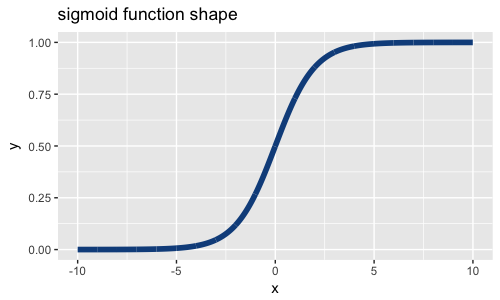
\includegraphics[width=.75\linewidth]{img/sigmoid.png}
  \caption{Sigmoid function. The domain of this function is $(-\infty, \infty)$ and the range $(0,1)$}
  \label{img:sigmoid1}
\end{figure}

Now, for the Rasch models, we need to analyse further the properties of the sigmoid function. If we subtract some positive scalar \textbf{a} to \textbf{x} in the equation \ref{eq:rasch1} then it result that the curve in \cref{img:sigmoid2} moves to the right, and the value of the sigmoid function decrease. Equivalently, if we add the same positive scalar \textbf{a}, then the curve moves to the left.

\begin{figure}[ht!]
  \centering
  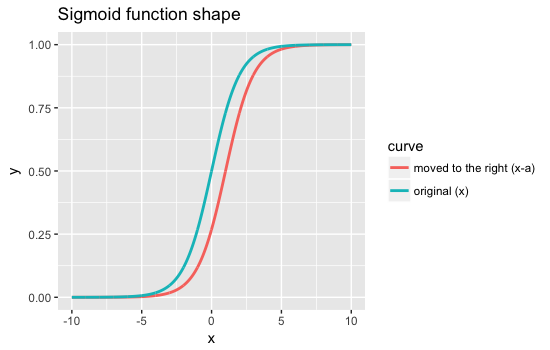
\includegraphics[width=.75\linewidth]{img/sigmoid_left.png}
  \caption{Effect of the variable \textbf{a} in the sigmoid function.}
  \label{img:sigmoid2}
\end{figure}


This idea is close to another formulation of the sigmoid function, which now can have two variables instead of one (\textbf{x,a}). With this modification, the domain and the range are the same. As mentioned before, the sigmoid function can be used to model a probability, that is, a continuous variable in the range [0,1], so then it is equivalent to a regression problem \footnote{More generally of a generalized linear model} \cite{friedman2009elements}. Now in terms of a classification problem (binary or dichotomous variable), this can be interpreted as the probability to belong to one of the two classes \footnote{Further generalizations for the polytomous case can be done.}. Then, the expression can be expressed as:

\begin{equation}
\begin{aligned}
\label{eq:rasch2}
 P(y = 1 | x,a) =& \frac{1}{1+\exp(-(x-a))} \\[2.5ex]
 =& \frac{\exp(x-a)}{1+\exp(x-a)}
\end{aligned}
\end{equation}

Where y is the binary variable. This basic idea is what support the basics of the Rasch model for dichotomous data.

\subsection{Rasch model}
Now, given this background, we can proceed with the definition of the Rasch model. From the last section, we can remember that the IRT models have a continuous latent variable (latent trait or ability) and an observable set of variables. In the next example, let's assume that this variable is binary and that the sigmoid function represents the probability of belonging to one of these classes.

\begin{equation}
  P(A_{rc} = 1 | \theta_r, \beta_c) = \frac{\exp(\theta_r - \beta_c)}{1+\exp(\theta_r - \beta_c)}
\end{equation}
Where:
\begin{itemize}
\item{$A$ is a matrix where the rows represent the persons and the columns the question of the quiz.}
\item{$A_{rc} \in \{0,1\}$ is the entry $(r,c)$ of the matrix $A$. This entry is a binary variable that represents the answer to the item $c$ of the person $r$. $0$ means that the person answers incorrectly and $1$ that answers correctly.}
\item{$\theta_r \in (-\infty, \infty)$ is the ability or trait of the person $r$.}
\item{$\beta_c \in [0, \infty)$ is the difficulty of the item $c$.}
\end{itemize}

Now, interpreting the result of the last subsection, if the parameter $\beta_c$ (difficulty) increases, then the sigmoid curve moves to the right leading to a decrease in the probability of getting correct the question. As in many statistical models, the problems rely on the parameter inference. For this reason, the author defines two auxiliary variables named \textit{Raw Scores}. Each of these scores is the marginalization of $A_{rc}$ with respect to the variables $r$ and $c$. Then each raw score depends only on one variable:

\begin{itemize}
\item{\textbf{Raw score per person:} $r_r = \sum_c A_{rc}$}
\item{\textbf{Raw score per item:} $s_c = \sum_r A_{rc}$}
\end{itemize}

The raw score per person is simply the sum of all the correct questions answered by each person; then it is a measure of the ability. On the other hand, the raw score per item is the sum of all persons that get correct that item, then it can be interpreted as the easiness of the item.

\subsection{The model assumptions}

According to \cite{demars2010item} \cite{mair2009extended} the Rasch model has the following assumptions:

\begin{itemize}
\item{ \textbf{1) Unidimensionality:}} The unidimensionality assumption is related to the dimensionality of the hidden parameters of the model. For the Rasch model, the ability parameter $\theta_{r}\in \mathbb{R}$ and the difficulty parameter $\beta_{c} \in \mathbb{R}$. Other models deal with multidimensional difficulty and ability parameters, but these will be not documented here.
\item{ \textbf{2) Conditional independence:}} The conditional independence is the same required for the latent variable models. This way, the observed item binary variables are independent among them given the parameters $\theta_{r}, \beta_c$
\item{ \textbf{3) Sufficiency of the raw score $r_r$:}} It is similar to the sufficiency in statistics. A statistics is sufficient if no other statistic provide some other information about the parameter with the sample.
\item{ \textbf{4) Monotonicity in the probability concerning the parameter $\theta_r$}}: That is, when having more ability, the probability of getting correct an item increase.

\end{itemize}

Due to the purpose of the text, the details about the tests for the assumptions will not be explained here. For more details about these tests, please consult \cite{demars2010item}.

\subsection{Item-parameter estimation}

In this section, a general review on the parameter estimation will be given. The basics of the item parameter estimation are based on the Maximum Likelihood Estimator, but according to \cite{mair2009extended} there are three ways to estimate the parameters:

\textbf{Joint Maximum likelihood Estimation (JML)}

The joint likehood formula of $\theta_r$ and $\beta_c$ is \cite{wright1969procedure} \cite{mair2009extended}:

\vspace{5 mm}

\begin{equation}
\begin{aligned}
L_{joint} =& \frac{\exp(\theta_r - \beta_c)^{\sum_c \sum_r a_{rc}}}{\prod_r \prod_i (1 + \exp(\theta_r - \beta_c))} \\[3.5ex]
    =& \frac{\exp(\sum_c \sum_r a_{rc} \theta_r) \exp(-\sum_c \sum_v a_{rc}\beta_c))}{\prod_r \prod_c (1 + \exp(\theta_r - \beta_c))} \\[3.5ex]
    =& \frac{\exp(\sum_r \theta_r r_r) \exp(-\sum_c \beta_c s_c)}{\prod_r \prod_c (1 + \exp(\theta_r - \beta_c))}
\end{aligned}
\end{equation}

\vspace{8 mm}

with $r_r = \sum_c A_{rc}$ and $s_c = \sum_r A_{rc}$. As reported in \cite{haberman1977maximum}, these estimation for the item parameters are not consistent when the number of the sample increases (there is one parameter per person, so it can increase too much).

\vspace{5 mm}

\textbf{Marginal Maximum likelihood Estimation (MML)}

If we integrate the person parameter, the joint distribution can be marginalised, and the parameters can be estimated via the Expected-Maximization algorithm \cite{bock1981marginal} \cite{mair2009extended}:

\vspace{5 mm}

\begin{equation}
L_{marg} = \prod_r \left[ \exp(-\sum_c \beta_c s_c) \int \frac{\exp(\theta_r)}{\prod_c^k (1 + exp(\theta-\beta_c)} dG(\theta)  \right]^{n_r}
\end{equation}

\vspace{5 mm}

Where it is assumed that the person parameter follows a predefined distribution. The expected maximisation algorithm is an algorithm that helps to maximise the likelihood of difficult problems. The idea is to include latent variables to make easier the maximisation process. For more information, this method is well documented in different texts \cite{friedman2009elements} \cite{bishop2006pattern}.

\vspace{5 mm}

\textbf{Conditional Maximum likelihood Estimation (CML)}

The third idea is to condition the joint likelihood on $r_r$ \cite{mair2009extended} (that is, conditioned on a sufficient statistic):

\vspace{5 mm}
\begin{equation}
L_{cond}= \frac{\exp(-\sum_r \beta_c s_c)}{\prod_r \sum_{x|r} ( -\exp(\sum_r x_r \beta_c)}
\end{equation}
\vspace{5 mm}

This way the parameters of the persons do not appear in the conditioning formula. 

\subsection{The Item Characteristic Curve (ICC)}

Now the question is how to plot the Rasch model. One way to do it is called the Item Characteristic Curve where we can display one item per curve. 

We already have the item and the person parameter, so we can calculate the probability of answering correctly one specific item for one specific person. If we make a plot where in the y-axis is the probability of getting correct this particular item and in the x-axis the person parameter and put one point per person. Then, the parameters of a sigmoid function are adjusted minimising the residuals between the individual points and this sigmoid function. This way we can have an Item Characteristic Curve as a representation of the model expectation \cite{demars2010item}:

\begin{figure}[ht!]
  \centering
  \includegraphics[width=.85\linewidth]{img/rasch_ICC.png}
  \caption{Item Characteristic Curve. Each curve represent one item.}
  \label{img:rasch_icc}
\end{figure}

The plot \cref{img:rasch_icc} plot is useful because we do not have to analyse all the abilities parameter of the persons, just one function that was fitted with all of these points. This way, we can easily identify which item was the most difficult. It is easy to identify that the leftmost curve is the easiest question and the rightmost curve the most difficult. 

\newpage

\subsection{The Person-Parameter plot (PPP)}
From the inference, we know the exact value of each person parameter, but now we have to answer how does this parameter be related to an observable variable. To answer this question, the Person-parameter plot maps the relation between the values of the ability parameter versus the number of correct answers of each person. This way we can have an idea of the relationship between the latent ability variable and the observable raw scores \cite{bond2015applying}:

\begin{figure}[ht!]
  \centering
  \includegraphics[width=.75\linewidth]{img/rasch_person.png}
  \caption{Rash model: person parameters. This plot shows the monotone relationship between the raw score per person and the value of the person parameter.}
  \label{img:rasch_person}
\end{figure}

\begin{table}[ht!]
\centering
\caption{Raw score per person and the person parameter.}
\label{tbl:person_pars}
\begin{tabular}{|l|l|l|}
\hline
\textbf{Person raw scores} & \textbf{\begin{tabular}[c]{@{}l@{}}Estimate person\\ parameter\end{tabular}} & \textbf{Std. Error} \\ \hline
5                         & -0.1963                                                                      & 0.6355              \\ \hline
6                          & 0.2050                                                                       & 0.6347              \\ \hline
7                          & 0.6182                                                                       & 0.6546              \\ \hline
8                          & 1.0750                                                                       & 0.7028              \\ \hline
9                          & 1.6339                                                                       & 0.8043              \\ \hline
10                          & 2.4685                                                                       & 1.0662              \\ \hline
\end{tabular}
\end{table}

In the \cref{img:rasch_person} we can see the raw scores and the person parameter from a synthetic dataset \footnote{the creation of this synthetic dataset are explained in chapter 4}. In this synthetic dataset, there were 11 questions, but the maximum raw score was 10. In the graph, we can observe that this relation is monotone. The idea is that between the number of correct answers increases, the student is more skilled.  \cite{bond2015applying}. 

\subsection{The Person-Item Map (PIM)}

Now, to show the relationship between the person parameters and the item parameters, the Person-Item map was created. In the uppermost part of this plot, it is shown the histogram of the person parameters regarding the latent dimension. We can see that the mode of this histogram was in the values $1.6339$ and $1.0750$ that correspond to eight and nine correct answers (see \cref{tbl:person_pars}). Also in the central part of the plot, we can observe the item parameters values (also regarding the same latent dimension).

This plot is interesting and useful because we can determine if the difficulty of the topics were lower for the ability of the students. In this synthetic example and the Person-Item map (\cref{img:rasch_personitem}), we can see that the difficulty of the topics are on the left side of the plot (most of them are below 0.6182 in the latent dimension), while the ability parameters of the students are in the right zone (most of them are above 0.6182 in the latent dimension). Then, in general terms in this example, the students were very skilled, and their ability was above the item difficulty. This is quite straightforward to deduce from the synthetic data set because to generate the answers, the probability to get right one question was at least 50\% for all items and students.

\begin{figure}[ht!]
  \centering
  \includegraphics[width=.75\linewidth]{img/rasch_personitem.png}
  \caption{Rasch model: Person-Item map}
  \label{img:rasch_personitem}
\end{figure}

\chapter{The lanalytics package}

The \textit{lanalytics package}\footnote{The package is open source and it is hosted on Github. \url{https://github.com/savrgg/lanalytics}} is an R package designed to analyse the answers to online quizzes. The objective of this package is to accomplish one of the main objectives of this text, that was the management and constant analysis of student answers and test times. The package is able to perform different analysis according to the desired grouping level: per quiz, per group and per person. To accomplish this, the data can be plotted in seven different ways, varying on the distinct aggregation levels and the different objectives of the analysis. At the group level, the package contains the \textit{guessing} and the \textit{Time-easiness} plots; at the quiz level, it contains two descriptive statistical graphs, a \textit{boxplot} and a \textit{histogram} of the obtained scores of the online quizzes takers and the \textit{Easiness-Time} and the \textit{Easiness-Time-Level} plots. Finally, at the individual level, the user can plot the grade history of a student. The explanations and objectives of each one of these will be explained throughout this chapter. For all the plots in this chapter, a synthetic dataset was used for illustration purposes; these plots were not generated with any real quiz dataset.

\section{Design of the package}

\subsection{Initial investigation}

Previous work on open source software for analysing quizzes has been done. One of the most popular software is Moodle (Modular Object Oriented Dynamic Learning Environment) that is learning management system \cite{zeileis2012flexible} \cite{moodle}. Which allows creating customisable webpages for the courses. With this tool, the instructors can generate and calculate the grades for their students. Also, it allows the tracking progress of the students. 

Some other user interfaces have been proposed to analyse the data from the students, as student engagement, attendance, and interactions with other students. For example, the Desire2Learn software has tools to achieve a personalised learning and also add-ons that allow analysing the engagement and the performance of the students \cite{desire}. Other software like learning catalytics was designed to increase student engagement  \cite{learningcatalytics}. But, as opposed to Moodle, these two solutions are not freely available.

In the CRAN (Comprehensive R Archive Network) there are some packages that allow the creation and evaluation of exams. One of these tools is the exams2nops function from the \textit{exams} package \cite{zeileis2012flexible}, but according to with the realized research no package was found to manage and analyze quizzes and items of the quizzes in distinct levels that was coded in R. For this reason, the lanalytics package was proposed as a useful tool to produce the required analysis for the instructors.

\subsection{Cognitive levels}

It is important to define the cognitive levels that are used in this package. These levels are based on the levels of the Bloom's taxonomy (remember, understand, apply, analyse, evaluate, create) \cite{Bloom1956}. The first level that we defined for this analysis include the easiest questions, those that only implies a \textit{factual knowledge}. These are questions that only require memorising and repeat the definition of a concept. The second level is the \textit{understanding of the concept}, where the student should not only know the definition but also to be able to discuss it and explain it. In the last level, \textit{application of concept}, the student should know how to execute and operate the concept in real problems or situations \cite{Stefan2015b}.

\subsection{Quiz and course objects}

To allow the instructors to manage the quizzes and course data, the lanalytics package created two exportable objects, the quiz object, and the course object. The basic structure of the lanalytics package is the quiz object which is implemented with a \textit{tibble} \cite{wickham2016r} \footnote{A tibble is data structure build on top of the data.frame class and give it more functionalities.}. This object contains a tibble in long format with one entry per student-question. For each row, another two variables are required: the score (a binary variable indicating if the answer was correct) and the date-time when the question was answered (in \textit{POSIXct} format). All this information should be provided in a \textit{*.csv} file. 

To allow more interesting analysis, the quiz object can be augmented with other two columns computed by R. The first is the spent time per question and the second is the answering order (a number is assigned to each row according to the order in which it was answered). An example of the quiz object is in the [\cref{img:quiz_object}]. 

\begin{figure}[ht!]
  \centering
  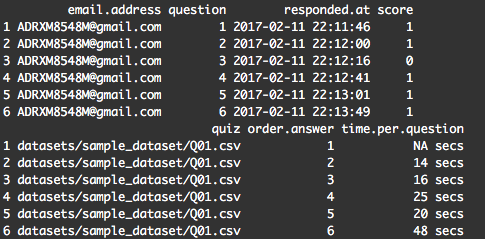
\includegraphics[width=.75\linewidth]{img/quiz_object.png}
  \caption{Quiz object. It has an specified format and columns.}
  \label{img:quiz_object}
\end{figure}

Finally, all the quizzes can be grouped in a course object, which joins them in the same tibble. This is very useful if the instructors want to save the all the records of their course in just one file.

\section{Group level analysis}
The group level analysis can potentially help the instructors to monitor the performance of all the group through all the course. Different interesting aspects of the group are analysed in this section. First, a guessing plot that helps to detect which potentially students that are answering randomly or with some exterior help is presented. After this, an Easiness-Time plot per time-terciles is made, in which the main objective is to understand in general how the group is answering the quiz regarding time. Also, the relation between this invested time and the obtained score in the items is presented. This tab was created to help the instructors to understand all the group behaviour in the quiz (for the guessing plot they can quickly observe the all the anomalous behaviours in the group and for the easiness time per quiz they can observe how the students are answering the questions according to the time).

\subsection{Guessing plot}

The idea of the \textit{guessing plot} \cite{Stefan2015b} [\cref{img:group_guess}] is to detect if a student is answering the questions in a very fast pace. Some students can answer the quizzes fast, but even the fastest of them answer the questions above some time threshold. This threshold is relative to the item difficulty and the student's ability, so one way to find a lower bound is to insert a question that every student can answer almost immediately in some section of the quiz and record the time that each student spends on it (For example, an easy a fast question can be: "did you attend this week's lecture?"). If some other question is answered below this time threshold, then it should be analysed. As the fast question answering does not give more information about the student behaviour (the student could be answering randomly or could know the answer from another student), the obtained score should be analysed. In the guessing plot if someone spends less time than the threshold, then a point will appear. If the answer was correct, then the colour of the point will be red. Otherwise, it will be blue.

\begin{figure}[ht!]
  \centering
  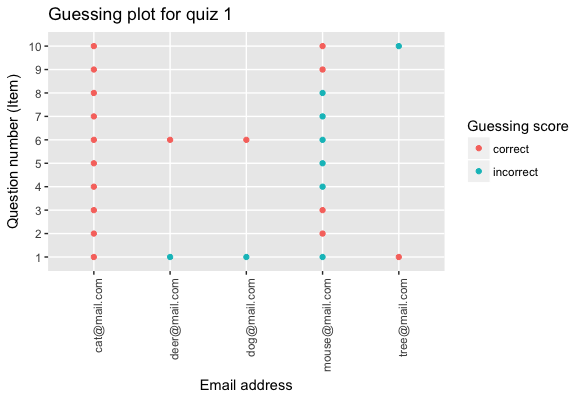
\includegraphics[width=.9\linewidth]{img/group_guess.png}
  \caption{Guessing plot. A point indicates that the user answers the item faster than some threshold. If it is red, the answer is correct, otherwise is incorrect.}
  \label{img:group_guess}
\end{figure}

The intuition of this plot is that, if the student gets many red points in the same quiz, it is possible that the answers to the items were known previous to the quiz. If the student gets many red and blue points, it is possible that the quiz was answered just randomly. The ideal situation is that no or just a few points appear per student in the graph. For example, in the \cref{img:group_guess} we have 5 users. The users \textit{cat@mail.com} and the user \textit{mouse@mail.com} answered fast all the questions, but the difference is that the user \textit{cat@mail.com} got every question correct while the other user does not. Because of the defined threshold, it is possible that the first student previously knew the answers, while the second one just answers randomly.


\subsection{Easiness time per quiz and tercils}

In the Easiness-Time plot \cref{img:group_order} the students are grouped by tertiles according to the time that they spent in the question. This way, the first tercile contains the fastest students and the third tercile the slowest. The intuition behind this plot is that, if both the fast and slow answering students score correctly in some question, then it is an easy one. On the other hand, if there is a score gap between the fast and slow students, then it may be interpreted differently. If the fast-answering students get a better result, then it may be interpreted as they know the solution, so they answer it faster. On the other hand, if the slow-answering students have a better result, this item might be a little bit confusing, so the students spend more time trying to figure out the solution.

\begin{figure}[ht!]
  \centering
  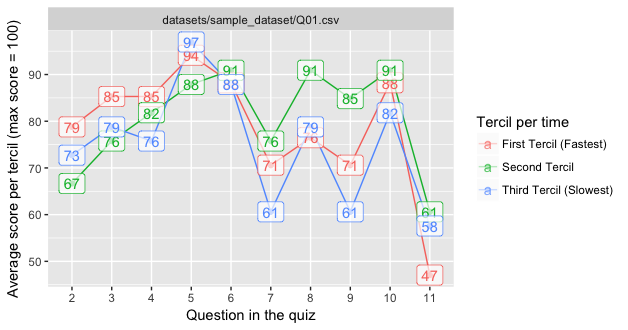
\includegraphics[width=\linewidth]{img/group_order.png}
  \caption{Easiness-Time per group and tercil. In the x-axis is the question of the quiz and in the y-axis the average score per time-tercil.}
  \label{img:group_order}
\end{figure}

In the \cref{img:group_order} we can see these patterns. For example, in the questions 5 and 6, all the students got an average of 90. Conversely, in the questions 2,3,4, the faster students got better results than, the slower ones.

\section{Quiz level analysis}

The quiz level analysis can potentially help the instructors to monitor the performance and analyse the data quickly from the perspective of the quiz and items. Different aspects that can be evaluated from this are the easiness of the items and the median spent time in each one of them \footnote{It has calculated the median so that the analysis is not affected by outliers}. First, to give a general idea of the performance of the students in the selected quiz, a histogram and a boxplot of the scores are displayed. This can help to analyse the outliers and the dispersion of the data. After these, two plots analyse the items from a perspective of easiness and time. Conversely to the Easiness-Time plot of the group level, here we are interested in the general performance of the quiz. We would like to observe that difficult items take more time than easy ones, so there is a negative relation between easiness and time. This point can be addressed with the ET-plot \cite{Stefan2015b}. Additionally, we would like to see if this easiness is related with the cognitive level, as intuitively, a higher cognitive level requires more time (For example, to apply a concept, first the student should understand it and remember it).

\subsection{Histogram of quizzes}

To identify the dispersion and skewness of the data we can analyse the histograms per quiz. With these is easy to detect if there are subpopulations in the data (for example if the distribution is similar to a bimodal normal distribution). In the [\cref{img:quiz_hist}] the quiz 01 looks normally distributed, and the quiz 02 looks like a bimodal distribution.

\begin{figure}[ht!]
  \centering
  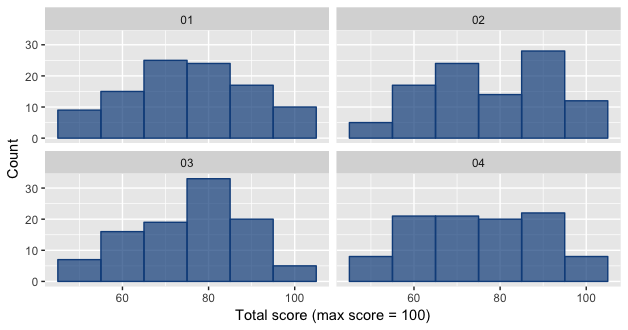
\includegraphics[width=.85\linewidth]{img/quiz_hist.png}
  \caption{Quiz scores histogram. In this plot four quizzes are displayed.}
  \label{img:quiz_hist}
\end{figure}

\subsection{Boxplot of quizzes}

Another way to verify the distribution and the skewness of the data is to analyse the boxplots of the scores. A useful aspect of these plots is that they allow us to detect outliers. This is important because the instructor can detect how many students are performing badly or well (depending on what kind of outlier is presented). After that, the instructor can only spend time analysing these points individually and see what topics are confusing for them.

The implemented boxplot in the ggplot2 package \cite{ggplot2} is the Tukey boxplots \footnote{Basically the other types of boxplots differ in the way that the whiskers are constructed.}, which use the first and third quartile as the hinges and limit the length of the whiskers to 1.5 of the interquartile IQR length. If a point in the data is outside these ranges, then it is classified as an outlier. For the upper whisker, if the value is greater than the maximum value of the data, then the whisker is reduced to this value (An equivalent rule apply for the lower whisker). 

\begin{figure}[ht!]
  \centering
  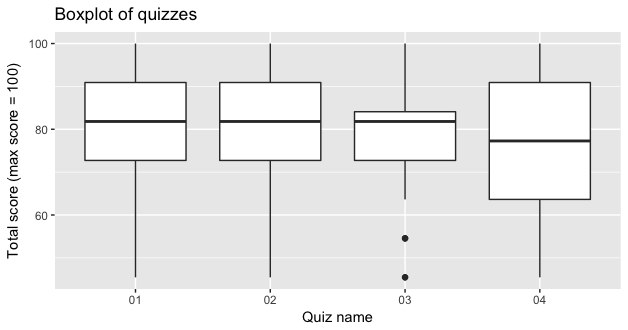
\includegraphics[width=\linewidth]{img/quiz_boxplot.png}
  \caption{Quiz scores boxplot (Also called box and whiskers diagram). This plot display five different summary statistics: median, two whiskers and two hinges. In addition the plot display the outlier points.}
  \label{img:quiz_boxplot}
\end{figure}

For example, in the boxplot of the \cref{img:quiz_boxplot} we can see that the lower whisker of the quiz 03 is much smaller than the other quizzes and, as seen in the histogram of the quiz 03, we can identify that this distribution has a much bigger mode than the other 3. As a consequence, the 50\% of the data is in contained in a smaller interval, which is reflected in its boxplot.

\subsection{Easiness-Time plot}

The objective of the Easiness-Time plot (ET plot) is to analyse the relationship between the required time for each item versus the average score obtained in the corresponding item. In the quiz design, it is important to consider the required time that each student should spend on each item, this way the instructor can design quizzes according to some pre-established time and discrimination criteria. With this plot, the instructor can analyse both points. Also, a tendency line is displayed in the plot.\footnote{To avoid overlay in the labels of the points; the ggrepel package was used.}.

\begin{figure}[ht!]
  \centering
  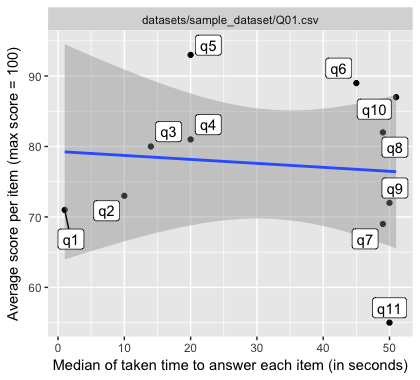
\includegraphics[width=.75\linewidth]{img/quiz_et.png}
  \caption{Easines-Time plot}
  \label{img:quiz_et}
\end{figure}

For example, in the \cref{img:quiz_et} we can see that question 5 is taking 20 seconds to answer (an intermediate time in this example), but the students achieve a high average score. On the other hand, the question 11 is taking too long for the students, and many of them get it wrong. Then, the instructor can examine why the students are getting wrong the question (because it seems that it is not a matter of time).

\subsection{Easiness-Time-Level plot}

The ETL plot \cite{Stefan2015b} adds the extra layer of the cognitive level to the ET plot. As stated at the beginning of the section, in this package we consider three different cognitive levels. The hypothesis is that difficult questions (in the sense of cognitive level) should take more time to answer than the easy ones. If we colour the points by the cognitive level, we might see that the high cognitive levels take in average more time to answer them (because we need to know the concept, then apply it). Moreover, in questions that require a high cognitive level, the students may get a lower score. The reasoning behind this idea is that, if the students don't know the factual knowledge (Low cognitive level), they will not know the application of this concept (High cognitive level), so the score is lower. 

The importance of this plot is to detect the questions where time and difficulty do not align with instructor-rated pre-established cognitive level. For example, if a low cognitive level question is taking too long to be answered, it could mean that this question is being difficult to understand or that the topic, in general, is difficult for the students (For example, in \cref{img:quiz_etl}, the question 6 and 10). Another example is the behaviour represented in question 1. This is a high cognitive question but the student answer it fast, so almost 30\% get it wrong. This can imply that the students have a misconception for the topic related to this question (the students think they know the answer, but they get it wrong). 

\begin{figure}[ht!]
  \centering
  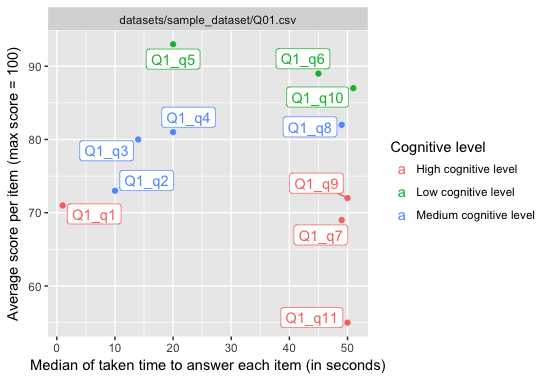
\includegraphics[width=.8\linewidth]{img/quiz_etl.png}
  \caption{Easiness-Time-Level plot.}
  \label{img:quiz_etl}
\end{figure}

\section{Individual plot}

Although the main objective of this package was to provide a way quickly analyse the data for all the group and quizzes, the instructors may be interested in visualising one particular student or group of students. In special if these students were outliers in the group and quiz analysis. This way, they can look for a specific way to support these students. To explore and understand the history of these particular students, an individual history plot is implemented. For this plot, the instructor needs to filter the required students from a list and then observe its history and scores in different quizzes. 

\begin{figure}[ht!]
  \centering
  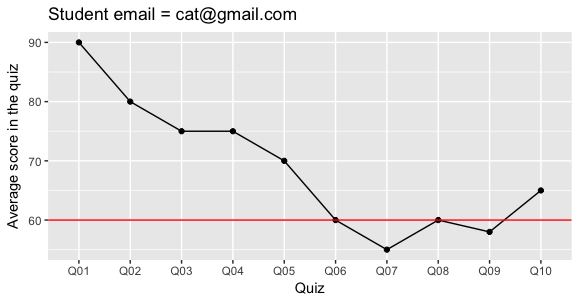
\includegraphics[width=\linewidth]{img/ind_student.png}
  \caption{Individual performance}
  \label{img:ind_student}
\end{figure}

Besides, when the course finishes, the instructor can upload a file with the final grade of the students and observe distinct patterns that can lead to failure of the test. An example of this graph is in the \cref{img:ind_student}. We can see that this student is getting worse in his evaluations, so an opportune instructor intervention in an early stage of the course could improve the student's performance on the final exam.

\section{Documentation}
Finally, the documentation is important for the package. For this reason, two different ways to make the documentation were compared. The first way, the codes were commented manually and then a document explaining how to call each function was created. This result to be an inefficient way because, in each change of the functions, both documents have to be modified. Then an alternative was considered. Then the roxygen2 package \cite{wickham5roxygen2} solves this problem. With this, it is only necessary to comment the codes with specific fields \footnote{it requires fields as title, description, parameters, return, examples, export} so that .R detect and compiles the documentation automatically. Also, it is very important this package because it facilitates the creation of the namespace and the exportable objects. Once used, .R automatically creates a \textit{.Rd} file for each function and saves it in the \textit{man} directory. 

To make more accessible the documentation, a webpage was considered. One way that works perfectly with the roxygen2 package is the pkgdown package, that helps us to create a website for the package (with the advantage that the examples in the documentation are executed and displayed). This package takes the generated documentation in the man directory and creates a webpage in the docs directory with the README file as the home page of the website. This structure works good with the free webpages storage of Github Pages, so it is used this way.
\chapter{Shiny interface}

Right now, the \textit{lanalytics} package is freely available from Github, but for people that are not R users, an interface should be implemented. The selected option is a Shiny dashboard \cite{shiny} \cite{chang2015shinydashboard} that contains the plots of the \textit{lanalytics} and the eRm packages. Shiny was selected because it is native to R (although it is a wrapper for HTML and CSS code). Also, it is designed to have the R console as backend (allowing to use any R package). 

The suggested dashboard contains five tabs related to distinct aspects of the \textit{lanalytics} package. In this chapter, a quick introduction of the design of the dashboard is provided, the theoretical justification, the technologies for the dashboard and the technical requirements. After that, the each tab will be explained in detail. The first tab only contains general instructions; the next two tabs are focused on importing and displaying the databases, while the last two tabs are focused on analysing the data in three different grouping levels. Furthermore, the last tab is used as an interface to the Rasch models of the eRm (extended Rasch model) package \cite{mair2009extended}. The usability of this Shiny Dashboard was evaluated with a focus group consisting of 3 people, but future evaluations with more people are suggested to make it usable for users in general.

As a reminder, the objective of the lanalytics package is to provide a tool for management and constant analysis of student answers and test times. Also, with the help of the eRm package, inferences related to the item difficulty and the abilities of the students is provided.

\section{Design of the dashboard}

\subsection{Initial investigation}

The idea behind this dashboard is that the instructors perform Just in Time Teaching and adapt their tests difficulties and necessities according to the specific group requirements. This idea is expressed in one of the five principles of social constructivism \footnote{In the literature, they use the idea that "Social constructivism emphasizes the importance of culture and context in understanding what occurs in society and constructing knowledge based on this understanding" \cite{kim2001social} \cite{mcmahon1997social}}: "A learning environment needs to be flexible and adaptable, so that it can quickly respond to the needs of the participants within" \cite{payne2009information} \cite{moodle}. Following this idea, and with the help of the \textit{lanalytics} and \textit{eRm}, the dashboard could be a tool that provides useful information to the instructor so that he takes his understanding of the group and the quizzes. 

\subsection{Technologies for a dashboard}

To create a Dashboard, there are distinct alternatives. For this dashboard, two software were studied. The first was Tableau Desktop, where the developers can easily create a dashboard without any programming background. The other analysed dashboard technology is the R Shiny software. This is based in the R-language, and you need to build the dashboard from scratch (Although there are packages that allow some predefined functions).

Tableau Desktop has many benefits. One of the principal is that different filters and rules between the filters can be applied very easily. Moreover, different pre-defined plots are available with just with a drag and drop feature. Also, it has the advantage that the Tableau dashboard can be viewed by everyone (just with the software installation), but to develop or modify a dashboard you need a license \footnote{although there is a free trial for the product}. For the connection to databases, you can connect Tableau to distinct sources of data, but this is a disadvantage for this particular project because the quiz data is stored in a CSV file or different formats. One major disadvantage of Tableau is that is only for visualisation purposes, so it is not possible to automatically apply a complex model in this software to the data.

On the other hand, \textit{shiny} is a web application framework that is native to R. In general, it is useful to create interactive applications, but if a dashboard is desired, an additional package should be installed. For the project, the \textit{shinydashboard} package was selected. The main advantage of this software is that is open source, and any application can be created. Besides, if some computation of a model is required, it is connected to the R console. Another main advantage of this software is that it allows the preprocessing of the files, allowing the flexibility to import quizzes from many formats \footnote{the current version only allows from R data format and CSV, although it is possible to create functions to use it with any input}.

\subsection{Requirements for Shiny}

Finally, to connect to the Shiny dashboard there are three alternatives: the first is to connect to the free service provided by RStudio in the website \textit{http://www.shinyapps.io/}, although this is limited by a monthly quota. The second way is to host it in Github and run it locally with the command \textit{runGitHub(repo = "savrgg/lanalytics", subdir = "shinyapp/")} and the third way is to clone the repository and run it locally. Due to the quota restrictions, it is suggested to run locally the project. To do it correctly, a prior installation of some packages need to be done: 

\begin{table}[ht!]
\centering
\caption{Required packages to run locally the lanalytics Dashboard}
\label{tbl:packages}
\begin{tabular}{|l|l|}
\hline
\textbf{Package} & \textbf{Usage}                                                                                                 \\ \hline
shiny            & \begin{tabular}[c]{@{}l@{}}Provides the functions to create interactive \\ applications.\end{tabular}          \\ \hline
shinydashboard   & \begin{tabular}[c]{@{}l@{}}Build on top of shiny, provides a template \\ for Dashboards.\end{tabular}          \\ \hline
DT               & \begin{tabular}[c]{@{}l@{}}Provides useful functions to display tables \\ and interact with them.\end{tabular} \\ \hline
tidyverse        & A collection of useful packages to analyze data.                                                               \\ \hline
stringr          & A package to manipulate strings.                                                                               \\ \hline
eRm              & A package that implements extended Rasch models.                                                               \\ \hline
ggrepel          & Functions to separate overlapping text labels.                                                                 \\ \hline
devtools         & Package with different tools for developers.                                                                   \\ \hline
\end{tabular}
\end{table}

\section{The lanalytics dashboard}

In R, under the Psychometric Models and Methods page, there are more than 40 statistical packages related to Item Response Theory. These are hosted in the CRAN across distinct servers and can be downloaded and used within R. Considering the realised investigation, two of the more useful for this project are the \textit{(latent trait models (ltm)} and the \textit{extended Rasch models (eRm)}. The first package implements the Rasch model, the two parameter logistic and the Birnbaum's Three-Parameter models. These include one or more of the following parameters: the difficulty of the items, the discrimination of the quiz and the guessing probability that a user had guessed a question \cite{rizopoulos2006ltm}. On the other hand, the eRm package has a different estimation procedure of the parameters and introduces tests to verify if the assumptions for the models are met \cite{mair2009extended}. These packages include many other models, but require that the users know how to code in R. This can be time-consuming for the instructors. 

\subsection{Content of the dashboard}

In this section, the main design for the dashboard is explored. As mentioned before, this consists of 5 different tabs that incorporate functions from the lanalytics and the eRm packages. All the screenshots of this chapter are in the appendix \ref{chap:screenshots}.

\vspace{4 mm}
\noindent{\textbf{Tab 1 and Tab 2: Instructions and import data tab}}
\vspace{2 mm}

As mentioned, the first tab contains the general instructions to operate the dashboard. Also, it contains a small explanation for the installation of the lanalytics package. This tab was designed just to introduce the user to the dashboard. The second tab contains input boxes for the quizzes files, the cognitive level file, and the final exam score file (optional). Shiny has the capability to upload many files at a time, but it should be opened in a web browser. Once a file is uploaded and the corresponding upload button is pushed, a list of the uploaded files will appear below the input boxes. The \cref{img:d_1}) contains an image of the first tab and the \cref{img:d_2}) of the import quizzes tab.

\vspace{4 mm}
\noindent{\textbf{Tab 3: Display quizzes tab}}
\vspace{2 mm}

The third tab (\textit{display quizzes}) was created to show the uploaded quizzes in the dashboard. First, it shows the quiz datasets; after that, the user has to select the columns for the cognitive levels file that contains the item and the corresponding cognitive level. Finally, the cognitive level file and in case that final exam results are uploaded, these are shown in the bottom of the page. To allow interactivity in the tables, such as filters and ordering, the DT package is used. This package is an interface to the DataTables library from JavaScript. The \cref{img:d_3_1} contains a screenshot of the design of this tab.

\vspace{4 mm}
\noindent{\textbf{Tab 4: Data analysis tab}}
\vspace{2 mm}

The fourth tab contains the quiz analysis tab. This is formed with another three sub tabs, each one of them representing distinct grouping level. 

\vspace{4 mm}
\noindent{\underline{Sub tab 1: Group analysis tab}}
\vspace{2 mm}

The first sub tab is the group analysis. First, in this group analysis, the quizzes to analyse have to be selected. Because of the nature of the plots, only one quiz at a time can be displayed. After the quiz is selected, two different plots are shown. As a reminder, the plots corresponding to the group level are the guessing plot \cref{img:d_4_1}  and the easiness-time per terciles  \cref{img:d_4_2}.

\vspace{4 mm}
\noindent{\underline{Sub tab 2: Quiz analysis tab}}
\vspace{2 mm}

In the second sub tab, the analysis at the quiz level is displayed. Similarly to the previous sub tab, the users have to select a quiz, only that in this tab, they can select one or more (although is suggested to select a few because it takes some time to plot many quizzes). In this tab, the boxplot of the scores, the histogram of the scores, the ET-plot and the ETL-plot are shown [\cref{img:d_5_1}, \cref{img:d_5_2}, \cref{img:d_5_3}]. This tab was designed so that the instructors could analyse all the items from the quiz in the same place.

\vspace{4 mm}
\noindent{\underline{Sub tab 3: Individual analysis tab}}
\vspace{2 mm}

In the last sub tab, it is shown the individual analysis. Here the users have a student email and also many quizzes analyse. If the final exam file is uploaded, then a red horizontal line will be plotted to show how the final grade was related to the grades from the quizzes. This is useful because the instructor can analyse the behaviour of the very good students or very bad students to understand how are they working through the course.

\vspace{4 mm}
\noindent{\textbf{Tab 5: Rasch model}}
\vspace{2 mm}

Finally, the last tab of the dashboard contains the plots related to the Rasch model. In this tab, the explained plots in chapter 2 are displayed. The ICC plot \cref{img:d_7_1}, the person-parameter plot \cref{img:d_7_2} and the person-item map \cref{img:d_7_3}] are provided. This way, the users can compare the difficulty of the items compared with the ability of the students.



\Chapter{Evaluation}

As stated in previous chapters, the Learning Analytics Software was created with two principal objectives. The first is to monitor the performance of the students in different levels: individual, per quiz and per group. The second is to ease the understanding of the items in online quizzes in order to improve the design of future quiz items \footnote{The second objective is focused on the understanding of the Item Response Theory.}. These two objectives were evaluated with a focus group that consisted of 3 persons working with online quizzes and interested in learning analytics topics. 

The general structure of the focus group consists of two big sections of 30 minutes each. The first was a general introduction to the Learning Analytics objectives, the implemented models and its capabilities. During this section a sheet of paper with a series of questions related to objective accomplishment was provided. The second 30 minutes of the focus group consisted of a user interface evaluation. 10 tasks were given and the participants had to evaluate some affirmations.

\section{Introduction of the software (30 minutes)}

This section of the focus group was divided into two parts, one of 10 minutes and the other of 20 minutes. The first part was used to introduce the capabilities of R and Shiny in order to motivate future uses and further implementations. The second part consisted of an introduction of the Learning Analytics Package objectives and its Shiny interface. In this phase the motivation of the models and the generated plots were explained.

As part of the evaluation five questions were asked in a sheet of paper for each of the participants. The objective was to discuss if the presented models were consistent with the objectives. The list of the five questions presented are the following:
  
  \begin{itemize}
\item{Do the shown figures in the \textbf{Individual analysis} help you to monitor how an individual student is performing? What else would you like to understand about the student?}
\item{Do the shown figures in the \textbf{Group analysis} help you to monitor how the group is performing?  What else would you like to understand about the group?}
\item{Do the shown figures in the \textbf{Quiz analysis} help you to understand the difficulty of the items as well as the required time per quiz? What are the main points that you consider when designing an item of a quiz?}
\item{The \textbf{Rasch model} helps you to understand the easiness-difficulty of your items?}
\item{The Rasch model plots \textbf{(ICC, Person-Item, Person-parameter)} gave you actionable information to improve the design of your quizzes?}
\end{itemize}

\section{User experience evaluation (30 minutes)}

Once the presentation of the software was concluded, the synthetic dataset was provided and a 20 minutes user experience evaluation started. In this part, the users had 10 tasks to accomplish [\cref{tbl:tasks}], with the central objective to evaluate the usability of the dashboard. In particular, they had to evaluate the easiness of the instructions as well as the easiness of the elements in the dashboard.

\begin{table}[ht!]
\centering
\caption{Tasks to accomplish}
\label{tbl:tasks}
\begin{tabular}{|l|l|}
\hline
\textbf{Tab}            & \textbf{Task}                                                                                                                     \\ \hline
Import quizzes tab      & Upload the quizzes files                                                                                                          \\ \hline
Import quizzes tab      & \begin{tabular}[c]{@{}l@{}}Upload the cognitive file and the final \\ exam file\end{tabular}                                      \\ \hline
Import quizzes tab      & Remove the cognitive file and upload it again                                                                                     \\ \hline
Display quizzes tab     & View if the uploaded files are correct                                                                                            \\ \hline
Display quizzes tab     & \begin{tabular}[c]{@{}l@{}}Select the Item and the Cognitive level column \\ for the cognitive file.\end{tabular}                 \\ \hline
Individual Analysis tab & Search one student and view its grades.                                                                                           \\ \hline
Group Analysis tab      & \begin{tabular}[c]{@{}l@{}}Select one quiz and view the guessers and \\ order plot\end{tabular}                                   \\ \hline
Quiz Analysis tab       & Observe the histogram and boxplot.                                                                                                \\ \hline
Quiz Analysis tab       & \begin{tabular}[c]{@{}l@{}}Observe the ET and ETL plot. Do you see \\ some pattern with the cognitive level?\end{tabular}         \\ \hline
eRm package tab         & \begin{tabular}[c]{@{}l@{}}Select one file and view the ICC, the person \\ item map and the person, parameters plot.\end{tabular} \\ \hline
\end{tabular}
\end{table}

To measure the usability of the dashboard, some affirmations were given and the users have to agree with them according to a Likert scale (1 = Strongly disagree, 2 = Disagree, 3 = Neutral, 4 = Agree, 5 = Strongly agree) [\cref{tbl:likert1}].

\begin{table}[ht!]
\centering
\caption{Likert evaluations}
\label{tbl:likert1}
\begin{tabular}{|l|l|l|l|l|l|l|}
\hline
\textbf{Tab}        & \textbf{Question}                                                                                                       & \textbf{SD} & \textbf{D} & \textbf{N} & \textbf{A} & \textbf{SA} \\ \hline
Import Quizzes      & It is easy to upload files.                                                                                         & 1           & 2          & 3          & 4          & 5           \\ \hline
Import Quizzes      & It is easy to remove files.                                                                                             & 1           & 2          & 3          & 4          & 5           \\ \hline
Import Quizzes      & It is clear when a file is uploaded.                                                                                    & 1           & 2          & 3          & 4          & 5           \\ \hline
Import Quizzes      & It is clear when a file is removed.                                                                                     & 1           & 2          & 3          & 4          & 5           \\ \hline
Display quizzes     & It is clear the format of the quizzes.                                                                                  & 1           & 2          & 3          & 4          & 5           \\ \hline
Display quizzes     & \begin{tabular}[c]{@{}l@{}}It is clear how to select the columns\\ of the cognitive file.\end{tabular}                  & 1           & 2          & 3          & 4          & 5           \\ \hline
Individual & \begin{tabular}[c]{@{}l@{}}It is easy to search for an student \\ email.\end{tabular}                                   & 1           & 2          & 3          & 4          & 5           \\ \hline
Individual & \begin{tabular}[c]{@{}l@{}}It is easy to visualize which quiz \\ is displayed in the plot.\end{tabular}                 & 1           & 2          & 3          & 4          & 5           \\ \hline
Individual & The plot is easy to read.                                                                                               & 1           & 2          & 3          & 4          & 5           \\ \hline
Group     & \begin{tabular}[c]{@{}l@{}}It is easy to visualize which quiz \\ is displayed in the plot.\end{tabular}                 & 1           & 2          & 3          & 4          & 5           \\ \hline
Group     & \begin{tabular}[c]{@{}l@{}}It is easy to identify possible guessing\\  or cheating misconducts.\end{tabular}             & 1           & 2          & 3          & 4          & 5           \\ \hline
Group     & \begin{tabular}[c]{@{}l@{}}It is easy to understand the relation of \\ time per question versus the grade.\end{tabular} & 1           & 2          & 3          & 4          & 5           \\ \hline
Quiz       & \begin{tabular}[c]{@{}l@{}}It is easy to visualize which quiz is \\ displayed in the plot.\end{tabular}                 & 1           & 2          & 3          & 4          & 5           \\ \hline
Quiz       & \begin{tabular}[c]{@{}l@{}}It is easy to interpret the histogram \\ and boxplot.\end{tabular}                           & 1           & 2          & 3          & 4          & 5           \\ \hline
Quiz       & \begin{tabular}[c]{@{}l@{}}The ET and ETL plots are easy \\ to interpret.\end{tabular}                                  & 1           & 2          & 3          & 4          & 5           \\ \hline
eRm         & \begin{tabular}[c]{@{}l@{}}The Item Characteristic Curve is \\ easily understandable.\end{tabular}                      & 1           & 2          & 3          & 4          & 5           \\ \hline
eRm         & \begin{tabular}[c]{@{}l@{}}The person-item plot is easily \\ understandable.\end{tabular}                               & 1           & 2          & 3          & 4          & 5           \\ \hline
eRm         & \begin{tabular}[c]{@{}l@{}}The person parameters are easily \\ understandable\end{tabular}                              & 1           & 2          & 3          & 4          & 5           \\ \hline

\end{tabular}
\end{table}

\newpage

After this, some general perceptions of the dashboard were asked (in the same likert scale) \cref{tbl:likert2}. 

\begin{table}[ht!]
\centering
\caption{Likert evaluations}
\label{tbl:likert2}
\begin{tabular}{|l|l|l|l|l|l|l|}
\hline
\textbf{Tab}        & \textbf{Question}                                                                                                       & \textbf{SD} & \textbf{D} & \textbf{N} & \textbf{A} & \textbf{SA} \\ \hline
General   & \begin{tabular}[c]{@{}l@{}}In general the models agree with the \\ general objectives\end{tabular}                      & 1           & 2          & 3          & 4          & 5           \\ \hline
General   & In general it is easy to use the buttons.                                                                               & 1           & 2          & 3          & 4          & 5           \\ \hline
General   & \begin{tabular}[c]{@{}l@{}}In general it is easy to navigate \\ between tabs.\end{tabular}                              & 1           & 2          & 3          & 4          & 5           \\ \hline
General   & \begin{tabular}[c]{@{}l@{}}In general the colors of the \\ dashboard are adequate.\end{tabular}                         & 1           & 2          & 3          & 4          & 5           \\ \hline
General   & In general the instructions are clear.                                                                                  & 1           & 2          & 3          & 4          & 5           \\ \hline
\end{tabular}
\end{table}

Finally, in the last section of the focus group, a final round of 10 minutes of open commentaries and suggestions was made. The objective of this final round was to provide a guideline for future work based on the different necessities of the users.

\section{Results}

In general, the qualitative result from this focus group was favorable for the package, just minor issues and further capabilities were suggested. Concerning the user interface, it needs to be improved in order to make it user-friendly and suitable for all kinds of audiences. More detailed areas of improvement are:
  
  \begin{table}[ht!]
\centering
\caption{My caption}
\label{tbl:improvements1}
\begin{tabular}{|l|l|}
\hline
\textbf{Analysis}   & \textbf{Ideas to improve}                                                                                                           \\ \hline
Individual analysis & \begin{tabular}[c]{@{}l@{}}- Allow the user to display multiple students in \\ the same plot\end{tabular}                           \\ \hline
Group analysis      & \begin{tabular}[c]{@{}l@{}}- Include a plot indicating the group average \\ score in all quizzes (not only by tercils)\end{tabular} \\ \hline
Rasch model         & \begin{tabular}[c]{@{}l@{}}- Needs better explanation to make interpretable \\ and actionable the results.\end{tabular}             \\ \hline
\end{tabular}
\end{table}

\newpage
Now, we can see the Likert evaluation of the tasks in the \cref{img:likert}. It is important to say that only 3 people were in the focus group, so the confidence interval that is displayed is only to show the variability for these persons.

\begin{figure}[ht!]
\centering
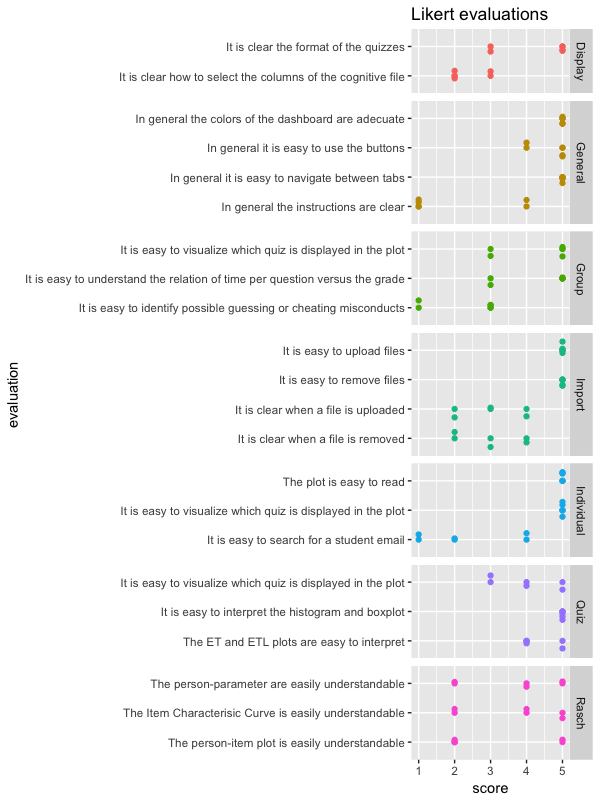
\includegraphics[width=\linewidth]{img/likert.png}
\caption{Evaluations in likert scale with a confidence interval of 1.5 standard deviation. Only 3 persons were in the focus group, then the lines are only for reference.}
\label{img:likert}
\end{figure}


From these evaluations and the commentaries from the focus group we can conclude four main points:
  
  \begin{itemize}
\item{In terms of the content in the plots, these display good and useful information} 
\item{There are some minor issues with the dashboard usability that can be improved}
\item{The rasch model should be explained in a more detailed way}
\item{The instructions shoud be more clear and detailed}
\end{itemize}

By analyzing the qualitative and the Likert evaluations, we can give more detailed areas of improvement. Concerning the lanalytics package, the majority of the plots were useful, but some suggestions were given to improve them. Some of them were as put some filters or additional characteristics, like being able to display more students in the same graph. 

For the user interface evaluations, useful insights were given. There are tabs where it is not intuitive what to do (in special the box related to the cognitive file import and the buttons to upload files) and some instructions are not clear.

For the third point, the Rasch model is a complex topic that should be explained in a much more detailed way. Currently, the instructions given in this section are not enough. Also, there should be more examples and interpretation of the parameters.

The fourth is the one that can improve a lot. It was suggested that the instructions should be more clear and explicit. Also they suggested that there should be one button that displays more detailed instructions and information. In addition it was suggested that a native English speaker proofread the dashboard in order to make the instructions clearer.







\chapter{Conclusions}
In this dissertation, the use of a tool for analysing low stake-high frequency quizzes was studied. Two objectives for this tool were proposed. The first was the measurement of the difficulty of the items and the abilities of the students, this with the objective to make more suitable the items according to the student abilities. And the second was to propose an open source tool that eases the administration and the analysis of these high-frequency quizzes. To make open source this project, the R language was selected. Finally, for the interactive dashboard, Shiny was selected over other dashboard visualisation tools like Tableau. 

In particular, for the first objective two packages for the Rasch models were explored. The first was the \textit{ltm} package that contains the 1-parameter logistic model (1PL) that contains a difficulty parameter, the 2-parameter logistic model (2PL) that contains, also, a discrimination parameter and the 3-parameter logistic model (3PL) that besides contains a guessing parameter. The second explored package was the \textit{eRm}, which contains the simple Rasch model that is similar to the 1PL. Also, it contains some useful plots to compare the item difficulty with the student abilities. Finally, for the included plots and the numerical stability, the eRm package was selected.

From the second point, the lanalytics package and the lanalytics dashboard were proposed, the package includes some basic descriptive analysis, while the dashboard includes the analysis of the lanalytics package and some plots of the eRm package. Initially, the software was thought to include quizzes from different input formats, but the variability of the inputs was too diverse that the homologation could be troublesome. In this aspect, the lanalytics package can be improved in a great sense. Right now the software accepts a specific *.csv format and also it accepts R data files. Also, the results can be output in .csv format and R data format. 

A focus group was made to evaluate if the objectives of the project were accomplished. In general, the evaluations for the content of the package and the dashboard were evaluated good, but there is a huge area of improvement on the instructions specification, on the provided examples and the explanation of the importance of each plot. Finally, the users agreed that the plots and the content agree with the general objectives of the project. For future work, a series of improvements in the usability should be done. This with the objective to make more attractive the software and to incentivise its use.
%% ... etc ...

%%%%%%%%
%% Any appendices should go here. The appendix files should look just like the
%% chapter files.
\appendix
\chapter{Screenshots of the dashboard}
\label{chap:screenshots}


\begin{figure}[ht!]
\centering
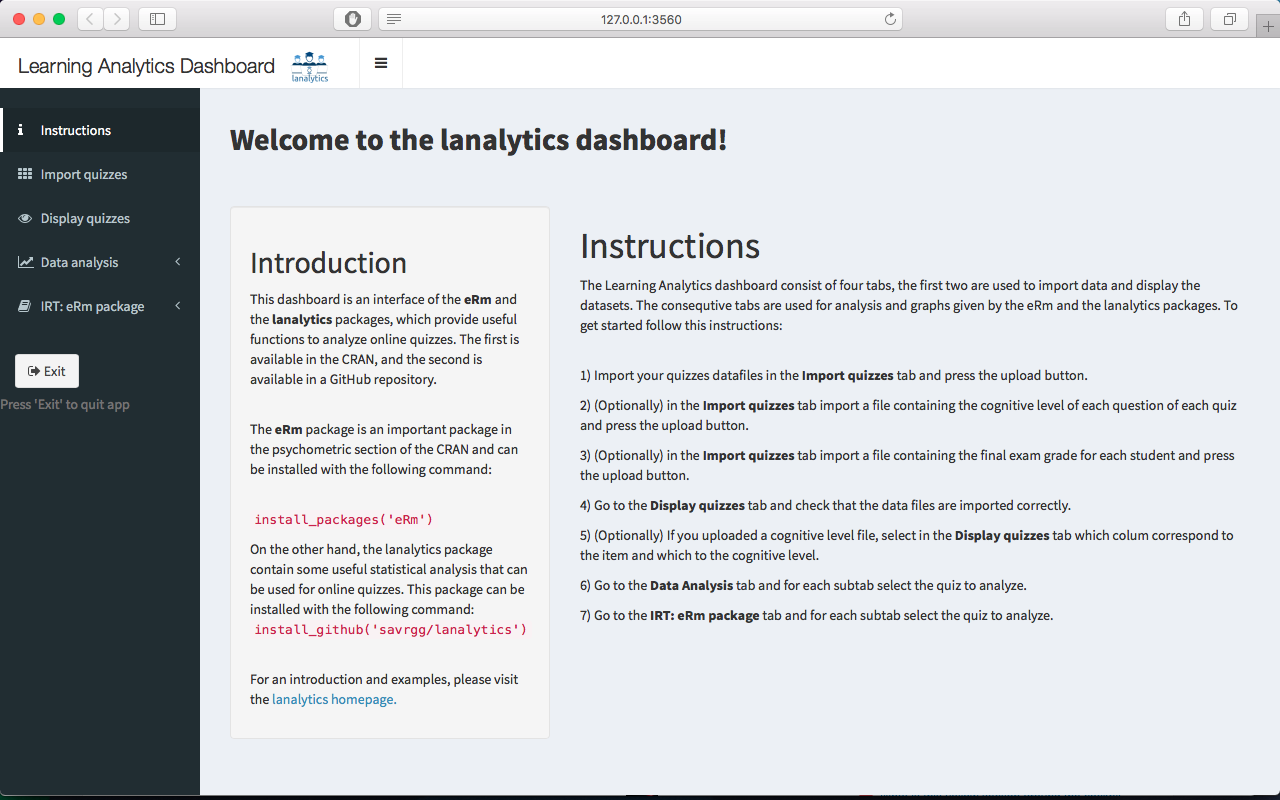
\includegraphics[width=\linewidth]{img/d_1.png}
\caption{Instructions tab}
\label{img:d_1}
\end{figure}

\begin{figure}[ht!]
\centering
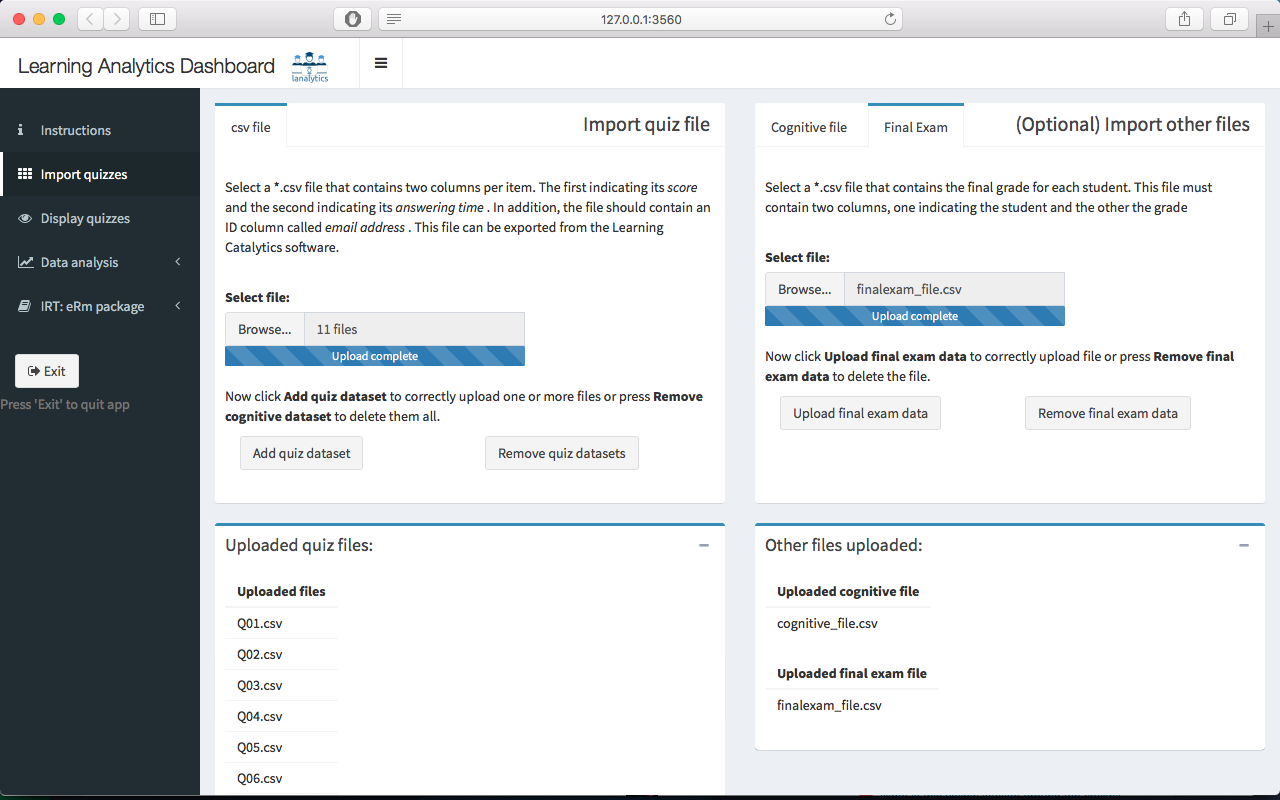
\includegraphics[width=\linewidth]{img/d_2.png}
\caption{Import data tab}
\label{img:d_2}
\end{figure}

\begin{figure}[ht!]
\centering
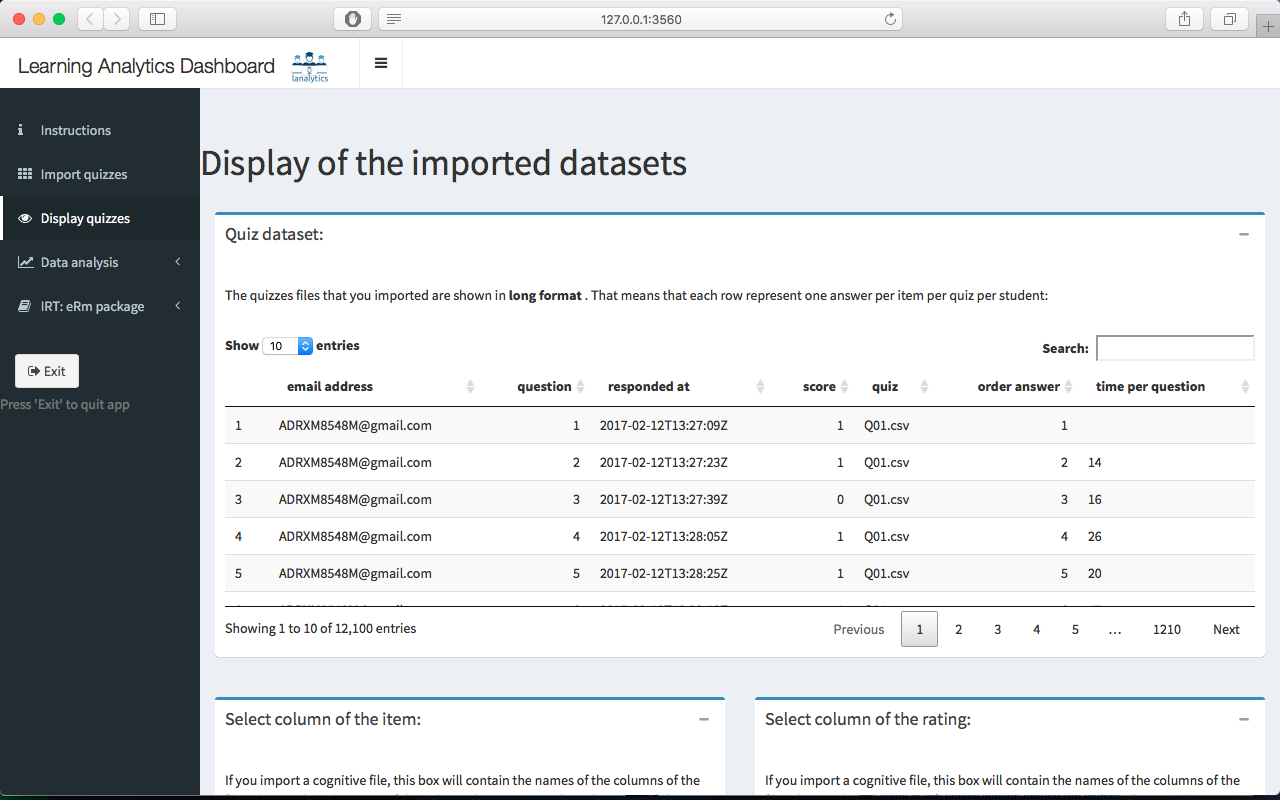
\includegraphics[width=\linewidth]{img/d_3_1.png}
\caption{Display quizzes tab}
\label{img:d_3_1}
\end{figure}

\begin{figure}[ht!]
\centering
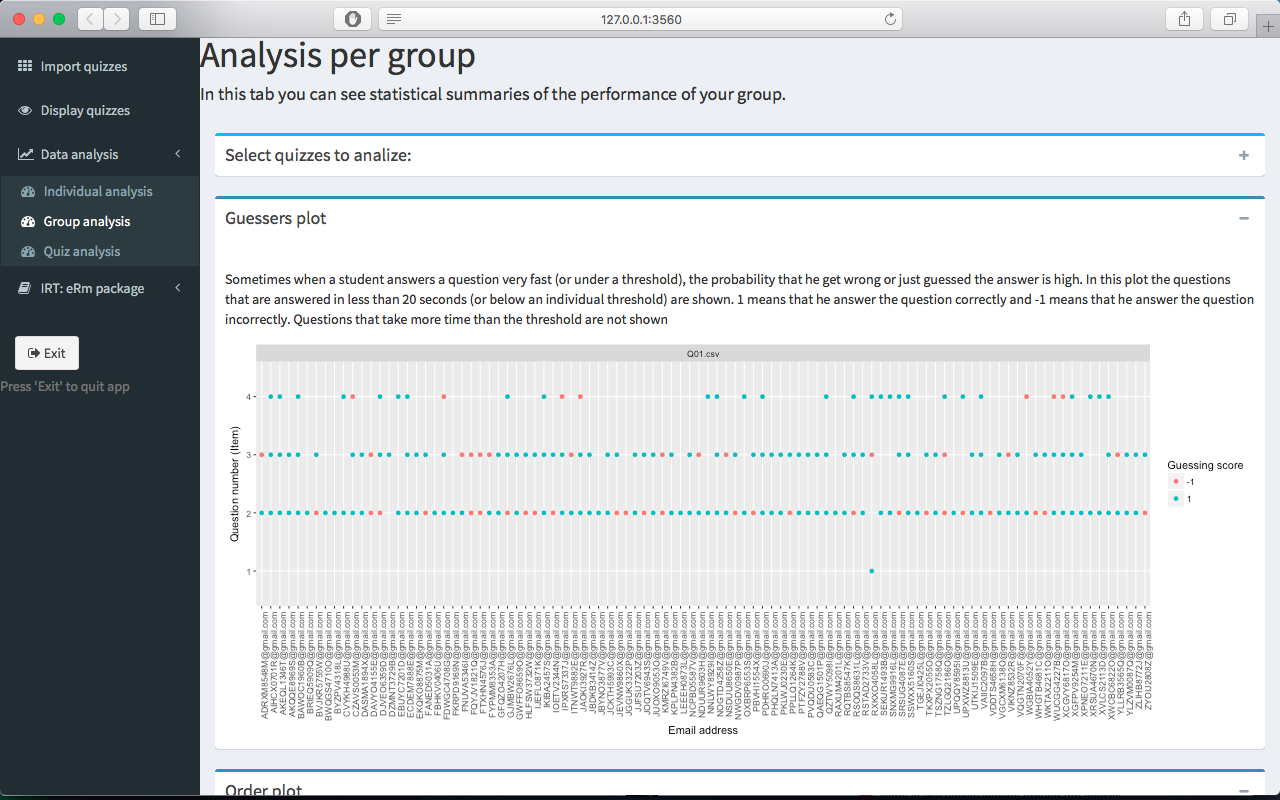
\includegraphics[width=\linewidth]{img/d_4_1.png}
\caption{Guessing plot}
\label{img:d_4_1}
\end{figure}
\begin{figure}[ht!]
\centering
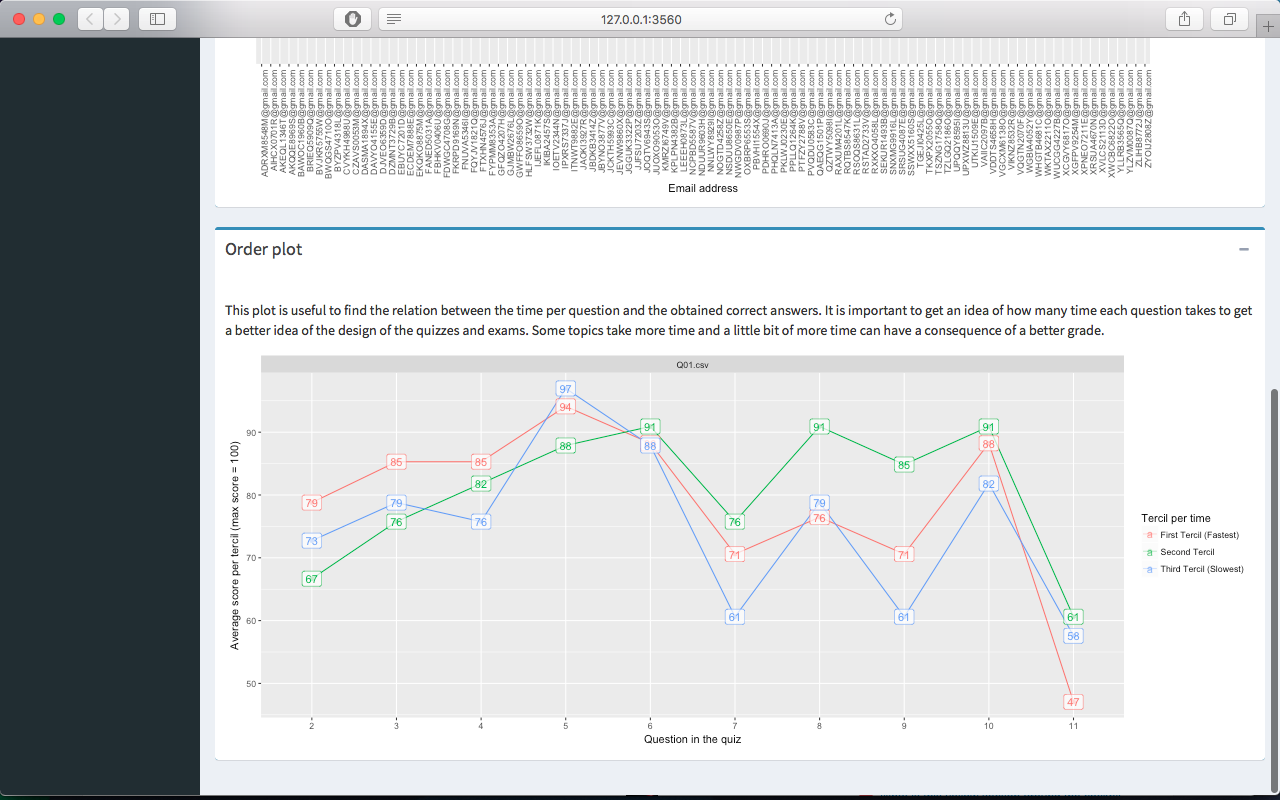
\includegraphics[width=\linewidth]{img/d_4_2.png}
\caption{Easiness-Time plot}
\label{img:d_4_2}
\end{figure}
\begin{figure}[ht!]
\centering
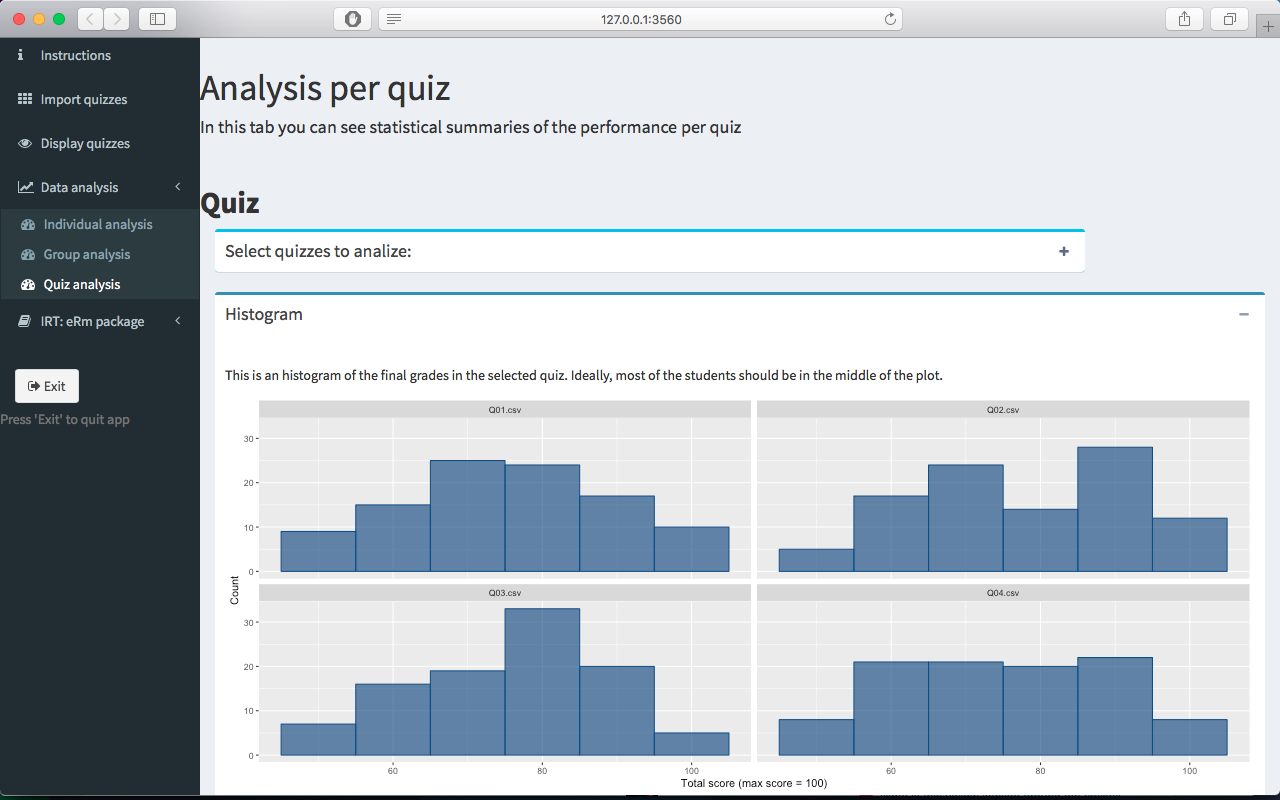
\includegraphics[width=\linewidth]{img/d_5_1.png}
\caption{Histogram of score per quiz}
\label{img:d_5_1}
\end{figure}
\begin{figure}[ht!]
\centering
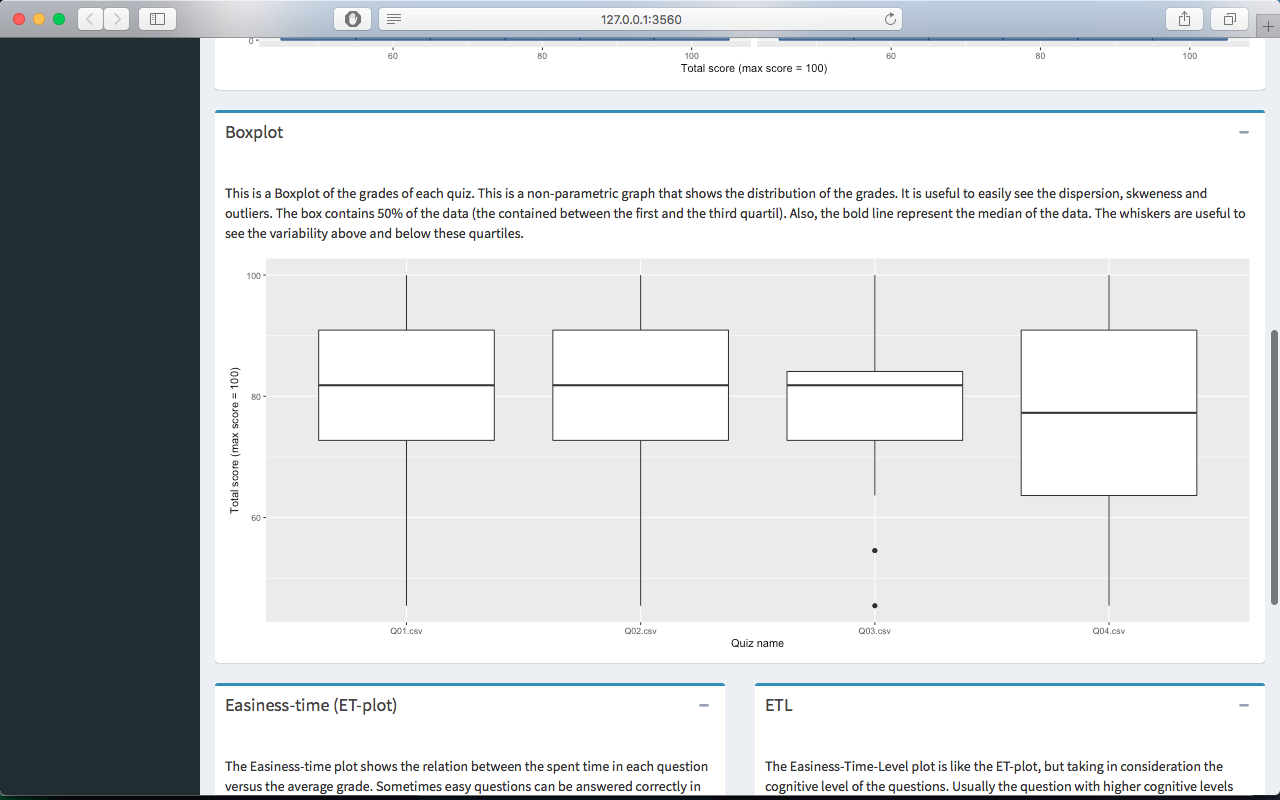
\includegraphics[width=\linewidth]{img/d_5_2.png}
\caption{Boxplot of score per quiz}
\label{img:d_5_2}
\end{figure}
\begin{figure}[ht!]
\centering
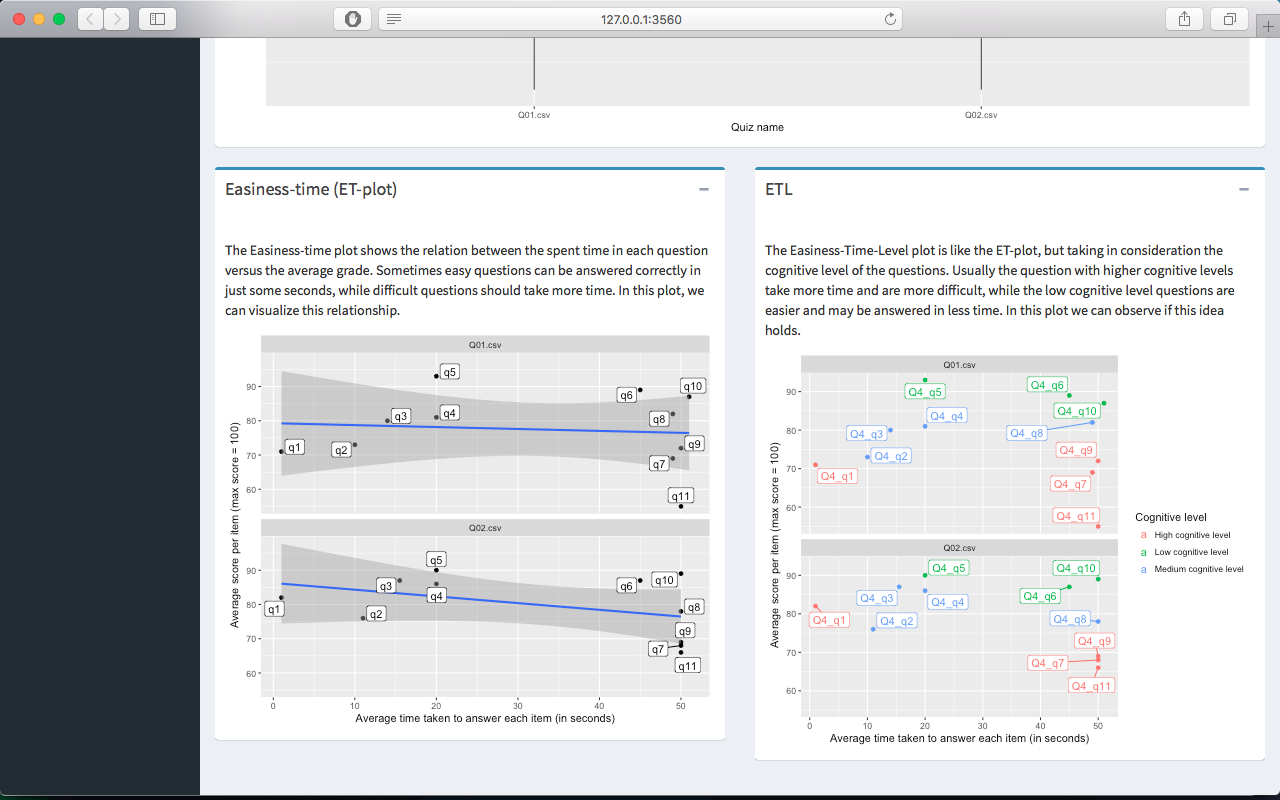
\includegraphics[width=\linewidth]{img/d_5_3.png}
\caption{ET and ETL plots}
\label{img:d_5_3}
\end{figure}
\begin{figure}[ht!]
\centering
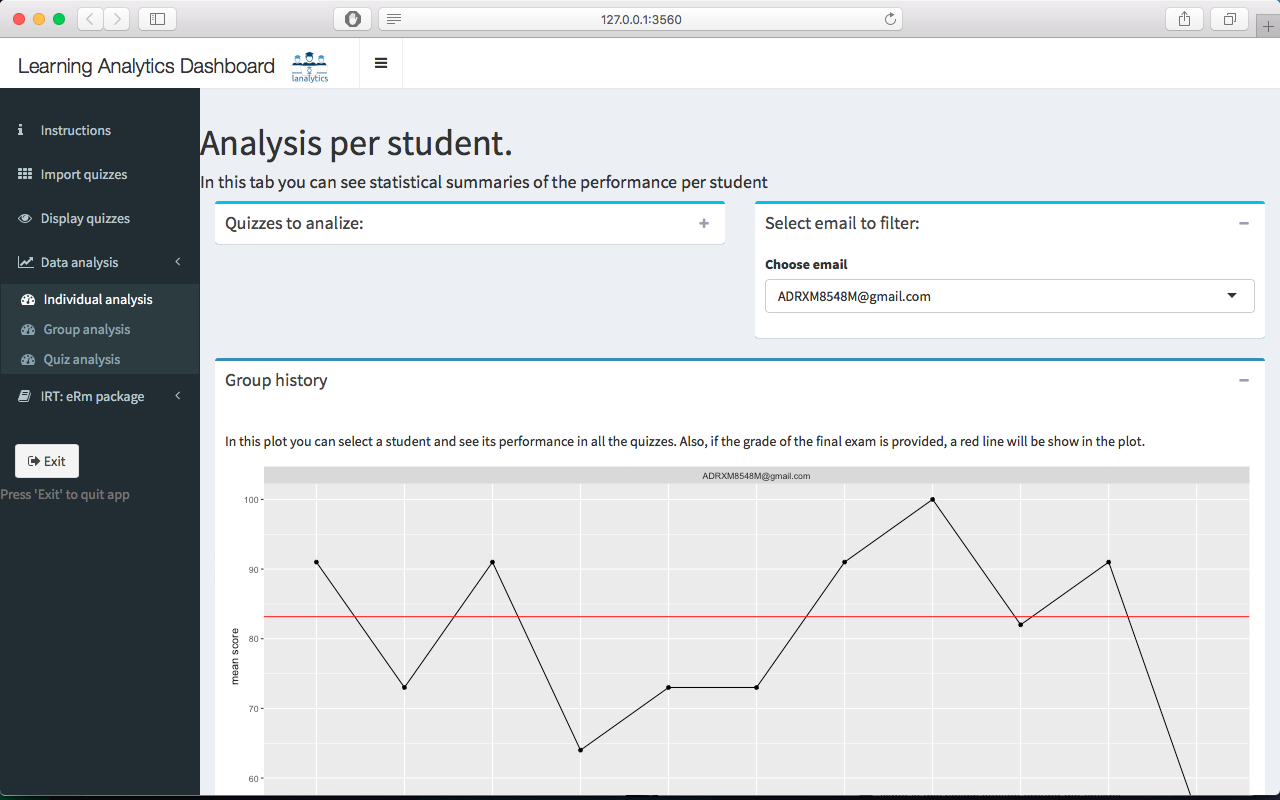
\includegraphics[width=\linewidth]{img/d_6.png}
\caption{Individual analysis tab}
\label{img:d_6}
\end{figure}

\begin{figure}[ht!]
\centering
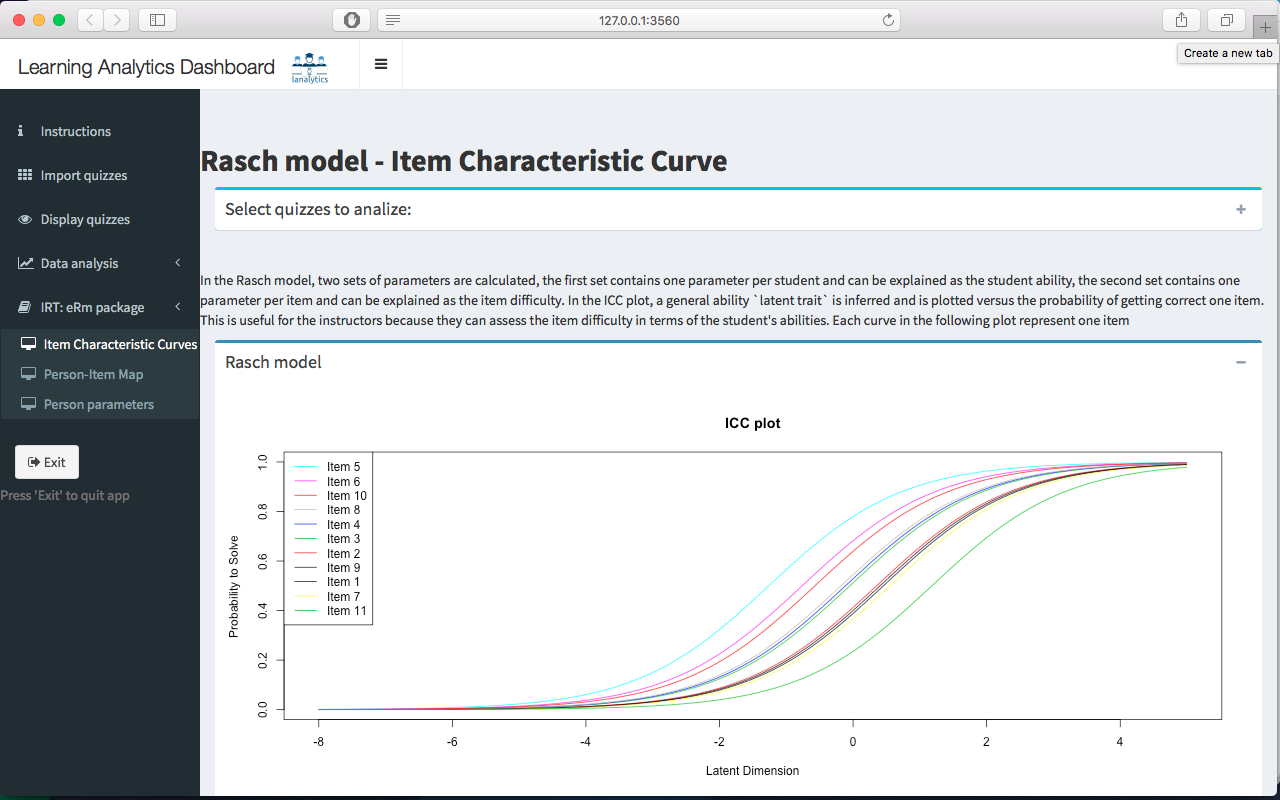
\includegraphics[width=\linewidth]{img/d_7_1.png}
\caption{Rasch model - ICC}
\label{img:d_7_1}
\end{figure}

\begin{figure}[ht!]
\centering
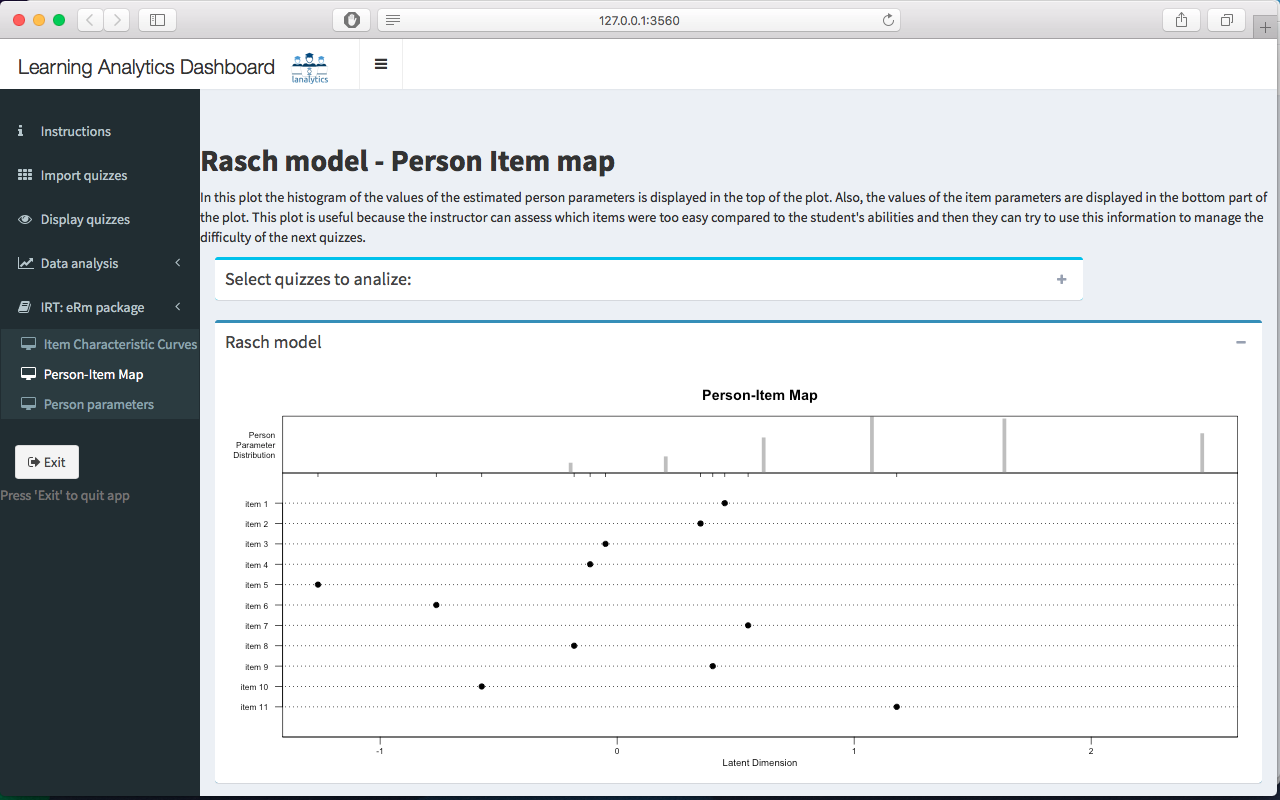
\includegraphics[width=\linewidth]{img/d_7_2.png}
\caption{Rasch model - Person Item map}
\label{img:d_7_2}
\end{figure}
\begin{figure}[ht!]
\centering
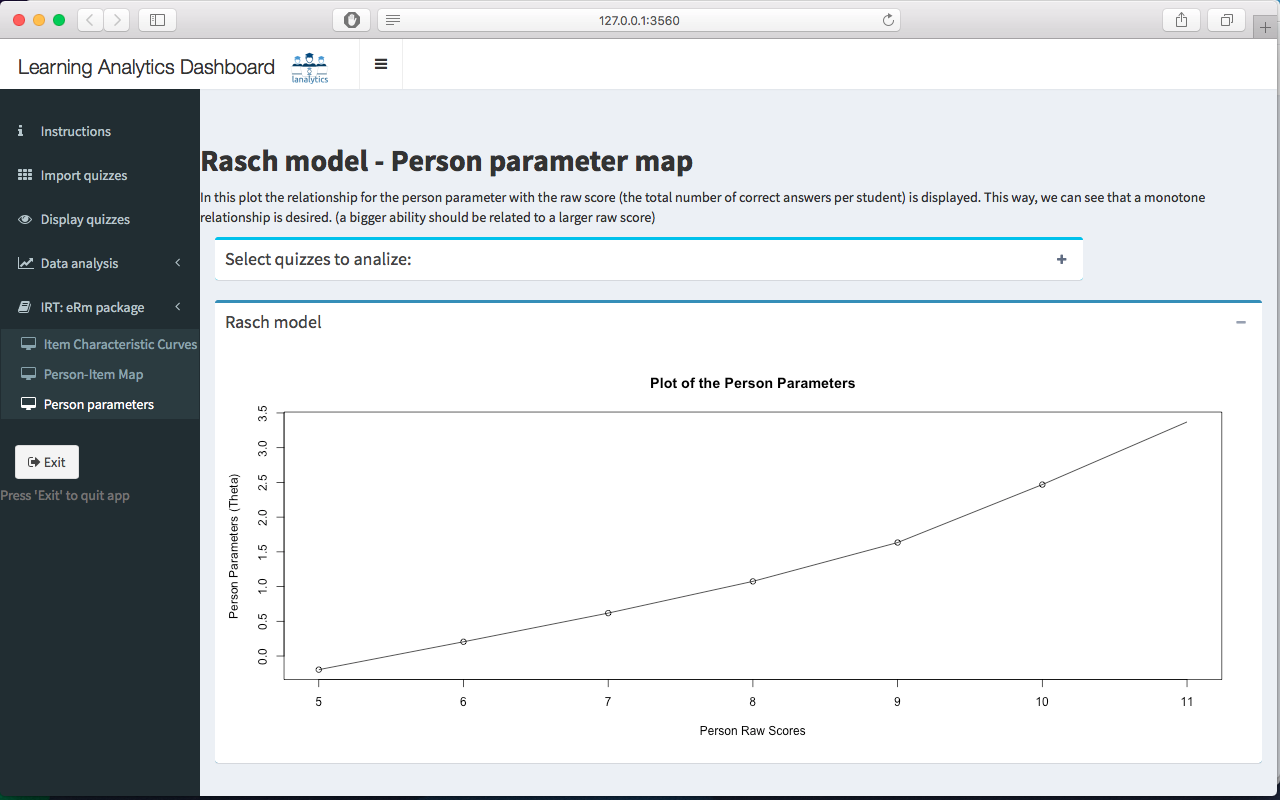
\includegraphics[width=\linewidth]{img/d_7_3.png}
\caption{Rasch model - Person parameter map}
\label{img:d_7_3}
\end{figure}




%% ... etc...

%% Choose your favourite bibliography style here.
\bibliographystyle{plain}

%% If you want the bibliography single-spaced (which is allowed), uncomment
%% the next line.
% \singlespace

%% Specify the bibliography file. Default is thesis.bib.
\bibliography{bibliography}

%% ... that's all, folks!
\end{document}
